\documentclass[11pt,paper=letter]{scrartcl}
\usepackage[wide,boxthm]{cjquines}

% socrery https://tex.stackexchange.com/a/69239/122245
\makeatletter
\newdimen\bibindent
\bibindent=16pt
\renewenvironment{thebibliography}[1]
  {\par\footnotesize
   \section*{\refname}
   \@mkboth{\MakeUppercase{\refname}}{\MakeUppercase{\refname}}
   \list{\@biblabel{\arabic{enumi}}}%
        {\settowidth\labelwidth{\@biblabel{#1}}%
         \leftmargin\labelwidth
         \advance\leftmargin\labelsep
         \advance\leftmargin\bibindent
         \itemindent -\bibindent
         \listparindent \itemindent
         \parsep \z@
         \usecounter{enumi}%
         \let\p@enumi\@empty
         \renewcommand\theenumi{\arabic{enumi}}}%
     \renewcommand\newblock{\hskip .11em \@plus.33em \@minus.07em}%
     \sloppy\clubpenalty4000\widowpenalty4000%
     \frenchspacing\footnotesize}
     {\endlist}
\makeatother

\let\faBoltOld\faBolt
\renewcommand{\faBolt}{{\relsize{-1}\faBoltOld}}

\begin{document}

\title{Obscure geometry theorems}
\author{Carl Joshua Quines}
\date{December 4, 2018}

\maketitle

\begin{abstract}

Any textbook goes through the proofs of Ceva's and Menelaus' theorems. But you haven't learned geometry through De Gua's or the radiation symbol theorem! In this handout, we'll discuss problem-solving techniques through the proofs of some obscure theorems.

\bluebf{More important than the theorems are their proofs and ideas}, and that's what we'll focus on. The theorems aren't that useful, but the techniques appear everywhere from short-answer to proof questions.

You should know about angle chasing, Ceva's and Menelaus' theorems, area ratios, similar and congruent triangles, the Pythagorean theorem, and parallelograms. Harder problems might need other geometry knowledge.

Each section ends with some questions related to the theorem, sorted by difficulty. Lightning bolts (\faBolt) mark harder problems. The problems range from pretty easy to olympiad-level questions; everyone from the beginner to the advanced reader should learn something useful.

Hints are available at the end. Use the hints one at a time: don't use the second until you've thought about the first. More problems, further reading, and references used in preparing the article are also at the end.

\end{abstract}

\section{Equilateral triangles}

Equilateral triangles seem like a boring subject for theorems. It's like trying to come up with theorems about squares. You get \emph{a square has equal diagonals} or \emph{a rectangle with three equal sides is a square}.

However, interesting things happen once we start adding other stuff. For example, the \href{https://en.wikipedia.org/wiki/British_flag_theorem}{British flag theorem} starts with a rectangle $ABCD$, but adds a point $P$.

\begin{probboxed}
  If you haven't heard of this theorem before, try proving it! Given a rectangle $ABCD$ and a point $P$ inside it, prove $AP^2 + CP^2 = BP^2 + DP^2$. \hint{\ref{h:bf11}}
  \begin{center}
    \begin{asy}
      size(5cm);
      pair A = (0, 0);
      pair B = (2, 0);
      pair C = (2, -1);
      pair D = (0, -1);
      pair P = (0.5, -0.4);
      draw(A--B--C--D--cycle);
      draw(A--P--B);
      draw(C--P--D);
      label("$A$", A, NW);
      label("$B$", B, NE);
      label("$C$", C, SE);
      label("$D$", D, SW);
      label("$P$", P, N);
    \end{asy}
  \end{center}
\end{probboxed}

Our first two theorems also have a similar setup: take an equilateral triangle $ABC$, and add a point $P$. Also like the British flag theorem, these two theorems talk about the lengths of $AP$, $BP$, and $CP$. Let's go!

\subsection{Van Schooten's theorem}

Try to prove the following theorem, or at least, draw some diagrams and convince yourself it's true:

\begin{probboxed}[van Schooten's theorem] Let $P$ be a point on the minor arc $BC$ of equilateral triangle $ABC$. Then $PA = PB + PC$.
\begin{center}
  \begin{asy}
    size(5cm);
    pair A = dir(90);
    pair B = dir(210);
    pair C = dir(330);
    pair P = dir(250);
    draw(circumcircle(A,B,C));
    draw(A--B--C--cycle);
    draw(A--P);
    draw(B--P--C);
    label("$A$", A, N);
    label("$B$", B, SW);
    label("$C$", C, SE);
    label("$P$", P, SW);
  \end{asy}
\end{center}
\end{probboxed}

If you know \href{https://en.wikipedia.org/wiki/Ptolemy\%27s_theorem}{Ptolemy's theorem}, then you should see a quick solution by applying it to quadrilateral $ABPC$. We'll try to prove this theorem without using Ptolemy's, instead making some clever constructions. 

To prove that $PA$ is the sum of $PB$ and $PC$, let's try to split up $PA$ into two segments. One will have length $PB$, and the other should have length $PC$. We pick the point $D$ on segment $PA$ such that $PD = PB$. Hopefully, the equal segments should produce some coincidences in our diagram.

\begin{center}
  \begin{asy}
    size(5cm);
    pair A = dir(90);
    pair B = dir(210);
    pair C = dir(330);
    pair P = dir(250);
    pair D = IP(circle(P, distance(B, P)), A--P);
    draw(circumcircle(A,B,C));
    draw(A--B--C--cycle);
    draw(A--D, bluey);
    draw(P--C, bluey);
    draw(B--D--P);
    draw(P--B);
    label("$A$", A, N);
    label("$B$", B, SW);
    label("$C$", C, SE);
    label("$P$", P, SW);
    label("$D$", D, NW);
  \end{asy}
\end{center}

From construction, we have $PD = PB$, so to finish, we need to prove $AD = PC$. Let's look at what we can get from $PD = PB$. If we draw $BD$, it doesn't just look like triangle $BDP$ is isosceles, but it looks like it's equilateral too. Try to prove this!

\begin{exboxed}
  Prove that triangle $BDP$ is equilateral. \hint{\ref{h:vs01}}
\end{exboxed}

An angle chase shows $\angle BPD = \angle BPA = \angle BCA = 60\dg$. Since $\triangle BDP$ is isosceles, the remaining two angles are $60\dg$, making it equilateral.

Maybe we can show that $AD = PC$ by constructing a similar equilateral triangle. Let $E$ be the point such that $\triangle ADE$ is equilateral. But there's a problem: there are \emph{two} possible choices of $E$ on opposite sides of $AD$. Let's draw both and see what happens.

\begin{center}
  \begin{asy}
    size(6cm);
    pair A = dir(90);
    pair B = dir(210);
    pair C = dir(330);
    pair P = dir(250);
    pair D = IP(circle(P, distance(B, P)), A--P);
    pair E2 = rotate(60, D)*A;
    pair E1 = rotate(-60, D)*A;
    draw(circumcircle(A,B,C));
    draw(A--B--C--cycle);
    draw(A--D, bluey);
    draw(P--C, bluey);
    draw(C--E1);
    draw(B--D--P);
    draw(P--B);
    draw(A--E1--D);
    draw(A--E2--D);
    label("$A$", A, N);
    label("$B$", B, SW);
    label("$C$", C, SE);
    label("$P$", P, SW);
    label("$D$", D, SE);
    label("$E_1$", E1, E);
    label("$E_2$", E2, W);
  \end{asy}
\end{center}

Surprisingly, it looks like $E_1$ lies on the circumcircle! It even looks like $B$, $D$, and $E_1$ are collinear! It also seems that this line is parallel to $PC$, which would make $DE_1CP$ is a parallelogram. In fact, if it was a parallelogram, we'd be done. 

\begin{exboxed} Try to prove these:
  \begin{enumthin}
    \item[(a)] If $DE_1CP$ is a parallelogram, then $AD = PC$.
    \item[(b)] $DE_1CP$ is a parallelogram! \hints{\ref{h:vs02} \ref{h:vs03}}
  \end{enumthin}
\end{exboxed}

For the first one, if it was a parallelogram, then $PC = DE_1$ because they're opposite sides. But $DE_1 = AD$ because $\triangle ADE_1$ is equilateral, so that finishes the proof. The second one's a bit harder, and needs some more steps. If you didn't get the exercise, try to show them individually:
\begin{itemize}[itemsep=-0.7ex]
  \item \emph{$B$, $D$ and $E_1$ are collinear:} $\angle ADE_1 = 60\dg = \angle BDP$.
  \item \emph{$E_1$ lies on the circumcircle:} $\angle AE_1B = \angle AE_1D = 60\dg = \angle ACB$.
  \item \emph{$DE_1$ and $PC$ are parallel:} $\angle ADE_1 = 60\dg = \angle ABC = \angle APC$.
  \item \emph{$DP$ and $E_1C$ are parallel:} $\angle BE_1C = \angle BAC = \angle PAE_1 = 180\dg - \angle PCE_1$.
\end{itemize}

That finishes the proof! We can write a nicer one if we directly construct the line parallel to $PC$ to define $D$ and $E$, rather than using equilateral triangles:

\begin{probboxed}
  Let the line through $B$ parallel to $PC$ intersect segments $AP$ and the circumcircle at points $D$ and $E$, respectively.
  \begin{enumthin}
    \item[(a)] Show that $\triangle BDP$ is equilateral, so $BP = DP$. \hint{\ref{h:vs04}}
    \item[(b)] Show that $\triangle ADE$ is equilateral, so $AD = DE$.
    \item[(c)] Show that $DECP$ is a parallelogram, so $DE = PC$. \hint{\ref{h:vs02}}
    \item[(d)] Finish the proof!
  \end{enumthin}
\end{probboxed}

For the first, we get $$\angle DPB = \angle APB = \angle ACB = 60\dg \quad\text{and}\quad \angle DBP = 180\dg - \angle BPC = \angle BAC = 60\dg,$$ so $\triangle BDP$ is equilateral. Also, $$\angle AED = \angle AEB = \angle ACB = 60\dg \quad\text{and}\quad \angle ADE = \angle PDB = 60\dg,$$ so $\triangle ADE$ is equilateral. Finally, $$\angle DEC = \angle BEC = \angle BAC = \angle ABC = \angle APC = \angle DPC,$$ so $DP$ and $EC$ are parallel. But $DE$ and $PC$ are parallel by construction, so $DECP$ is a parallelogram. This gives $AP = AD + DP = DE + BP = PC + BP$.

The main trick in this proof is to \bluebf{divide a segment to show it's the sum of two others}. It appears in a lot of other problems as well, and I talk about this more in my other handout \href{http://cjquines.com/files/constructions.pdf}{Constructions}.

\begin{mdframed}[style=exmdbox]
  \begin{exercise}
    What happens when $P$ lies on minor arc $AB$ or minor arc $CA$ instead?
  \end{exercise}

  \begin{exercise}
    In the proof, we constructed the point $D$ on $AP$ such that $PB = PD$. What would happen if we construct the point $D$ on $AP$ such that $PC = PD$ instead? Does the proof still work? What would need to be changed?
  \end{exercise}

  \begin{problem}[\faBolt \! \cite{ctkvanschooten}]
    In $\triangle BPC$, $\angle BPC = 120\dg$. Let $Q$ be the foot of the angle bisector of $P$ to $BC$. Prove that $PQ(BP + PC) = BP \cdot PC$. \hints{\ref{h:vs31} \ref{h:vs32}}
  \end{problem}

  \begin{problem}[\faBolt\! \href{https://aops.com/community/c6h58299}{IMO 1997}]
    Angle $A$ is the smallest in triangle $ABC$. Points $B$ and $C$ divide the circumcircle of the triangle into two arcs. Let $U$ be an interior point of minor arc $BC$. The perpendicular bisectors of $AB$ and $AC$ meet line $AU$ at $V$ and $W$, respectively. Lines $BV$ and $CW$ intersect at $T$. Show that $AU = TB + TC$. \hints{\ref{h:vs41} \ref{h:vs42}}
  \end{problem}
\end{mdframed}

\subsection{Pompeiu's theorem}

Van Schooten's theorem dealt with the case when $P$ is on the circumcircle of $\triangle ABC$. We're left with the case when $P$ \emph{isn't} on the circumcircle. This is covered by our next theorem, Pompeiu's theorem:

\begin{probboxed}[Pompeiu's theorem] Let $P$ be a point \emph{not} on the circumcircle of an equilateral triangle $ABC$. Then there exists a triangle with side lengths $PA$, $PB$, and $PC$. 
\begin{center}
  \begin{asy}
    size(7cm);
    pair A = dir(90);
    pair B = dir(210);
    pair C = dir(330);
    pair P = dir(180)*0.3;
    pair D1 = rotate(60, P)*B;
    draw(A--B--C--cycle);
    draw(A--P, ruddy);
    draw(P--B, greeny);
    draw(P--C, bluey);
    transform t = shift(2, -0.1)*rotate(203);
    draw(t*C--t*P, bluey);
    draw(t*P--t*D1, greeny);
    draw(t*C--t*D1, ruddy);
    label("$A$", A, N);
    label("$B$", B, SW);
    label("$C$", C, SE);
    label("$P$", P, NW);
  \end{asy}
\end{center}
\end{probboxed}

Let's try the same thing we did for van Schooten's theorem, and \emph{construct a triangle with these side lengths}. Let's use $PC$ as one of the sides and add a point $D$ so that $\triangle PCD$ has the side lengths we want. Then $DP$ and $DC$ should have the same lengths as $PA$ and $PB$, in some order.

There are four possibilities, and two of them make sense. Of course, we don't know if either one exists, but let's assume it does and see what we get.

\begin{center}
  \begin{asy}
    size(5cm);
    pair A = dir(90);
    pair B = dir(210);
    pair C = dir(330);
    pair P = dir(180)*0.3;
    pair D1 = rotate(60, P)*B;
    pair D2 = rotate(-60, P)*A;
    draw(A--B--C--cycle);
    draw(A--P, ruddy);
    draw(P--B, greeny);
    draw(P--C, bluey);
    draw(C--D1, ruddy);
    draw(P--D1, greeny);
    draw(C--D2, greeny);
    draw(D2--P, ruddy);
    label("$A$", A, N);
    label("$B$", B, SW);
    label("$C$", C, SE);
    label("$P$", P, NW);
    label("$D_1$", D1, S);
    label("$D_2$", D2, N);
  \end{asy}
\end{center}

The first possibility is $D_1$ such that $D_1P = PB$ and $D_1C = PA$. The other one is $D_2$ such that $D_2P = PA$ and $D_2C = PB$. Either one makes sense because they make an isosceles triangle: in the first case, you have $\triangle BPD_1$; in the second case, you have $\triangle APD_2$. Like last time, it seems that we have some good coincidences:

\begin{exboxed}
  Assume that point $D_1$ exists. Convince yourself that $\triangle BPD_1$ looks equilateral. Using this, show that $\triangle CBD_1 \cong \triangle ABP$.
\end{exboxed}

If $\triangle BPD_1$ were equilateral, then we'd get $BD_1 = BP$. We also have $D_1C = PA$ by construction, and $CB = AB$. So by SSS congruence, we get $\triangle CBD_1 \cong \triangle ABP$. These are great coincidences, if we only knew that $D_1$ existed in the first place!

Here's a general trick. Suppose you want to show a point $P$ with property $A$ also has property $B$. Then try constructing a point $P'$ such that it has property $B$ in the first place, then show that $P' = P$! In other words, \bluebf{add a phantom point}! 

So instead of starting with a point $D_1$ such that $\triangle PCD_1$ has the side lengths we want, we'll start with a point $D$ such that $\triangle BPD$ is equilateral, and hope we still have $\triangle CBD \cong \triangle ABP$!

\begin{center}
  \begin{asy}
    size(5cm);
    pair A = dir(90);
    pair B = dir(210);
    pair C = dir(330);
    pair P = dir(180)*0.3;
    pair D1 = rotate(60, P)*B;
    draw(A--B--C--cycle);
    draw(A--P, ruddy);
    draw(P--B, greeny);
    draw(P--C, bluey);
    draw(C--D1, ruddy);
    draw(P--D1, greeny);
    draw(B--D1, greeny);
    label("$A$", A, N);
    label("$B$", B, SW);
    label("$C$", C, SE);
    label("$P$", P, NW);
    label("$D$", D1, S);
  \end{asy}
\end{center}

\begin{exboxed}
  Construct $D$ such that triangle $BPD$ is equilateral, as in the diagram. Show that $\triangle CBD \cong \triangle ABP$. Then finish the proof! \hint{\ref{h:pt01}}
\end{exboxed}

We can't use SSS congruence, since we don't know if $CD = AP$. In fact, that's what we're trying to prove, so we definitely can't use that! But we still have $BD = BP$ and $CB = AB$. So we only need to show $\angle CBD = \angle ABP$. Some angle chasing shows us that $\angle CBD = \angle PBD - \angle PBC = \angle ABC - \angle PBC = \angle ABP,$ so we're done by SAS congruence! The congruence gives us $CD = AP$, and then $\triangle PCD$ has the side lengths we want.

There's another, important way to look at triangles $CBD$ and $ABP$. They're related through a \bluebf{rotation}. Indeed, consider a $60\dg$ rotation centered on point $B$: it takes $P$ to $D$ and $A$ to $C$, so those triangles must be congruent! The idea of rotating to match up segments appears in the following exercises too.

\begin{mdframed}[style=exmdbox]
  \begin{exercise}
    Does the proof still work when $P$ is outside of $ABC$? What happens when $P$ is on the circumcircle? How does this relate to van Schooten's theorem?
  \end{exercise}

  \begin{exercise}
    Point $O$ is on the plane of an equilateral triangle $ABC$ such that $\angle AOC = 90\dg$ and $\angle BOC = 75\dg$. Find the angles of the triangle with sides $AO$, $BO$, and $CO$.
  \end{exercise}

  \begin{problem}
    Point $P$ is inside square $ABCD$ such that $PA = 1$, $PB = 2$, and $PC = 3$. Find $\angle APB$. \hints{\ref{h:pt41} \ref{h:pt42}}
  \end{problem}

  \begin{problem}[\faBolt]
    Point $P$ is inside equilateral triangle $ABC$ such that $PA = 3$, $PB = 4$, and $PC = 5$. Find the area of triangle $ABC$. \hints{\ref{h:pt31} \ref{h:pt32}}
  \end{problem}

  \begin{problem}[\faBolt\! \faBolt\! \href{https://s3.amazonaws.com/hmmt-archive/november/2018/HMMTNovember2018GeneralRoundSolutions.pdf}{HMMT 2018}]
    Equilateral triangle $ABC$ has circumcircle $\Omega$. Points $D$ and $E$ are chosen on minor arcs $AB$ and $AC$ of $\Omega$ respectively such that $BC = DE$. Given that $\triangle ABE$ has area $3$ and $\triangle ACD$ has area $4$, find the area of $\triangle ABC$. \hints{\ref{h:pt51} \ref{h:pt52} \ref{h:pt54} \ref{h:pt53}}
  \end{problem}
\end{mdframed}

\subsection{Viviani's theorem}

This two previous theorems dealt with the distances from a point to the vertices. Viviani's theorem, on the other hand, deals with the distances from a point to the \emph{sides} of the triangle. 

\begin{probboxed}[Viviani's theorem] Let $P$ be a point inside equilateral triangle $ABC$. Then the sum of the distances from $P$ to the sides of the triangle is equal to the length of its altitude. 

\begin{center}
  \begin{asy}
    size(5cm);
    pair A = dir(90);
    pair B = dir(210);
    pair C = dir(330);
    pair P = dir(200)*0.3;
    draw(A--B--C--cycle);
    draw(P--foot(P,A,B), ruddy);
    draw(P--foot(P,B,C), greeny);
    draw(P--foot(P,C,A), bluey);
    real x = distance(P, foot(P,A,B));
    real y = distance(P, foot(P,B,C));
    real z = distance(P, foot(P,C,A));
    pair D = foot(A, B, C);
    draw(A--(A*(y+z)+D*x)/(x+y+z), ruddy);
    draw((A*(y+z)+D*x)/(x+y+z)--(A*(y+x)+D*z)/(x+y+z), greeny);
    draw(D--(A*(y+x)+D*z)/(x+y+z), bluey);
    label("$A$", A, N);
    label("$B$", B, SW);
    label("$C$", C, SE);
    label("$P$", P, N);
  \end{asy}
\end{center}
\end{probboxed}

Since we have altitudes, we're motivated to look at the areas of triangles. This is because the distance from $P$ to $BC$, for example, is an altitude:

\begin{exboxed}
  Consider the distance from $P$ to $BC$. Which triangle is it an altitude of? How does this relate to the triangle's area? Complete the proof.
\end{exboxed}

\begin{center}
  \begin{asy}
    size(5cm);
    pair A = dir(90);
    pair B = dir(210);
    pair C = dir(330);
    pair P = dir(200)*0.3;
    draw(A--B--C--cycle);
    draw(P--foot(P,A,B), ruddy);
    draw(P--foot(P,B,C), greeny);
    draw(P--foot(P,C,A), bluey);
    draw(A--P--B);
    draw(P--C);
    label("$A$", A, N);
    label("$B$", B, SW);
    label("$C$", C, SE);
    label("$P$", P, NW+(0,1.5));
    label("$a$", P--foot(P,B,C), E);
    label("$b$", P--foot(P,A,C), N);
    label("$c$", P--foot(P,A,B), SW);
  \end{asy}
\end{center}

If we let $a$ be the distance from $P$ to $BC$, and $s$ be the side length of $\triangle ABC$, then the area of $\triangle BPC$ is $\frac12 as$. Similarly, if we let $b$ and $c$ be the distances from $P$ to $CA$ and $AB$, the areas of $\triangle CPA$ and $\triangle APB$ are $\frac12 bs$ and $\frac12 cs$. But these areas add up to the area of $\triangle ABC$! If the height of $\triangle ABC$ is $h$, we get $$\frac{as}{2} + \frac{bs}{2} + \frac{cs}{2} = \frac{hs}{2},$$ and dividing both sides by $\frac 12 s$ gives $a + b + c = h$, so we are done.

The trick of \bluebf{considering areas} is something we'll develop more in the next section. 

\begin{mdframed}[style=exmdbox]
  \begin{exercise} \label{pr:vivianigeneralize}
    Does the theorem generalize to parallelograms? There's no sense of an ``altitude'', but is the sum of the distances from $P$ to the sides of the parallelogram constant? (\emph{Constant} means it doesn't change no matter which point $P$ we pick.) What about tetrahedrons? What about regular polygons, in general? 
  \end{exercise}

  \begin{exercise}
    Suppose that for a $\triangle ABC$, if we choose any point $P$ inside it, the sum of the distances from $P$ to the sides of the triangle is constant. Does it mean $\triangle ABC$ is equilateral? \hint{\ref{h:vt21}}
  \end{exercise}

  \begin{problem}[\cite{wilsonviviani}]
    It's also possible to prove Viviani's theorem using constructions, like we did for the previous two theorems. Try to do so. This diagram might help:
    \begin{center}
      \begin{asy}
        size(6cm);
        pair A = dir(90);
        pair B = dir(210);
        pair C = dir(330);
        pair P = dir(200)*0.3;
        draw(A--B--C--cycle);
        draw(P--foot(P,A,B), ruddy);
        draw(P--foot(P,B,C), greeny);
        draw(P--foot(P,C,A), bluey);
        real x = distance(P, foot(P,A,B));
        real y = distance(P, foot(P,B,C));
        real z = distance(P, foot(P,C,A));
        pair D = foot(A, B, C);
        draw(A--(A*(y+z)+D*x)/(x+y+z), ruddy);
        draw((A*(y+z)+D*x)/(x+y+z)--(A*(y+x)+D*z)/(x+y+z), greeny);
        draw(D--(A*(y+x)+D*z)/(x+y+z), bluey);
        B = dir(330);
        C = dir(210);
        real sh = distance(foot(P,B,C), B) - distance(P,foot(P,B,C))/sqrt(3);
        pair Ap = A - (sh, 0);
        pair Bp = B - (sh, 0);
        pair Cp = C - (sh, 0);
        draw(Ap--Bp);
        draw(C--Cp--Ap);
        draw(foot(P,A,C)--foot(P,Ap,Cp), bluey);
        pair Q = Ap - (0, x) - (0, z);
        draw(Ap--Q);
        draw(foot(P,A,D)--(2*Q-P), linetype(new real[]{6, 4}));
      \end{asy}
    \end{center}
  \end{problem}

  \begin{problem}[\faBolt\! \href{https://www.amt.edu.au/wp-content/uploads/15AIMO.pdf}{Australian Intermediate 2015}]
    Point $X$ is chosen inside an equilateral triangle $ABC$, and $Y$, $Z$, and $W$ are the feet of the perpendiculars from $X$ to $AC$, $AB$, and $BC$, respectively. It is given $XY : XZ : XW = 1 : 2 : 4$. Find the ratio of the areas of $AZXY$ and $ABC$. \hints{\ref{h:vt41} \ref{h:vt42}}
  \end{problem}

  \begin{problem}[\faBolt\,\faBolt \! \cite{abboudviviani}]
    Prove the extension to equiangular polygons: the sum of the distances from an interior point to the sides of an equiangular polygon is constant. \hints{\ref{h:vt51} \ref{h:vt52}} % pf: inscribe a regular polygon inside. 
  \end{problem}
\end{mdframed}

% https://arxiv.org/pdf/0903.0753.pdf provides an iff characterization.

\section{Ratios and areas}

Areas are a powerful tool. In the previous section, we used areas to give a short proof of Viviani's theorem. \href{https://en.wikipedia.org/wiki/Ceva\%27s_theorem}{Ceva's theorem} is another theorem that can be proven using areas. In particular, we'll look at \bluebf{area ratios}.

Here, we look at two theorems that both involve ratios of areas. We'll be referring to areas a lot in this section, so define $[ABCD]$ to be the area of quadrilateral $ABCD$, and $[ABC]$ to be the area of $\triangle ABC$. We'll start with a proof of Ceva's theorem.

\begin{probboxed}[Ceva's theorem]
  Let $P$ be a point inside triangle $ABC$. Let lines $AP$, $BP$, and $CP$ meet opposite sides at points $D$, $E$, and $F$, respectively. Then $$\frac{AF}{FB} \cdot \frac{BD}{DC} \cdot \frac{CE}{EA} = 1.$$

  \begin{center}
    \begin{asy}
      size(5cm);
      pair A = dir(110);
      pair B = dir(210);
      pair C = dir(330);
      pair P = incenter(A,B,C)*1.1;
      pair D = extension(A,P,B,C);
      pair Ep = extension(B,P,A,C);
      pair F = extension(C,P,A,B);
      draw(A--B--C--A);
      draw(A--D);
      draw(B--Ep);
      draw(C--F);
      label("$A$", A, dir(A));
      label("$B$", B, dir(B));
      label("$C$", C, dir(C));
      label("$D$", D, dir(D));
      label("$E$", Ep, dir(Ep));
      label("$F$", F, dir(F));
      label("$P$", P, NE+(0,1));
    \end{asy}
  \end{center}
\end{probboxed}

In the proof of Viviani's theorem, we used $[APB]$, $[BPC]$, and $[CPA]$. Here, we use the same trick. But as stated earlier, we look at their \emph{ratios}. Try this:

\begin{exboxed}
  Show that $\dfrac{[APB]}{[CPA]} = \dfrac{BD}{DC}$. Then finish the proof! \hints{\ref{h:cv01} \ref{h:cv02}}
\end{exboxed}

Here, we apply a very useful fact when dealing with area ratios. \bluebf{If two triangles have the same altitude, the ratio of their areas is the ratio of their bases.} Look at $\triangle ADB$ and $\triangle CDA$. They have the same altitude from $A$ to $BC$. Similarly, $\triangle PDB$ and $\triangle CDP$ share the same altitude from $P$ to $BC$. This gives us $$\frac{BD}{DC} = \frac{[ADB]}{[CDA]} = \frac{[PDB]}{[CDP]}.$$ How do we get $[APB]$? It looks ike $[ADB]$, but we subtract $[PDB]$. This is where we use a little algebraic trick: if $\frac ab = \frac xy$, then $\frac ab = \frac xy = \frac{a+x}{b+y}$. For example, since $\frac 23 = \frac 46$, both are equal to $\frac {2+4}{3+6} = \frac69$. Applying this gives us $$\frac{BD}{DC} = \frac{[ADB] - [PDB]}{[CDA] - [CDP]} = \frac{[APB]}{[CPA]}.$$ But now multiplying the similar results $\frac{AF}{FB} = \frac{[CPA]}{[BPC]}$ and $\frac{CE}{EA} = \frac{[BPC]}{[APB]}$ gives us the desired theorem.

The key idea in this proof is that \bluebf{triangles with shared altitudes have area ratios equal to base ratios}. We will use this fact over and over again in this section.

\subsection{One-seventh area triangle}

Before dealing with our next theorem, let's consider this special case:

\begin{probboxed}[One-seventh area triangle] In triangle $ABC$, points $D$, $E$, and $F$ lie on sides $BC$, $CA$, and $AB$ respectively, such that $$\frac{CD}{BD} = \frac{AE}{CE} = \frac{BF}{AF} = 2.$$ Then the area of the inner triangle formed by the lines $AD$, $BE$, and $CF$ is one-seventh the area of $ABC$.
  \begin{center}
    \begin{asy}
      size(5cm);
      pair A = dir(110);
      pair B = dir(210);
      pair C = dir(330);
      pair D = (2*B+C)/3;
      pair Ep = (2*C+A)/3;
      pair F = (2*A+B)/3;
      fill(extension(A,D,B,Ep)--extension(B,Ep,C,F)--extension(C,F,A,D)--cycle, opacity(0.2)+rgb(0.1,0.417,0.571));
      draw(A--B--C--A);
      draw(A--D);
      draw(B--Ep);
      draw(C--F);
      label("$A$", A, dir(A));
      label("$B$", B, dir(B));
      label("$C$", C, dir(C));
      label("$D$", D, S);
      label("$E$", Ep, NE);
      label("$F$", F, dir(F));
    \end{asy}
  \end{center}
\end{probboxed}

There's a lot of symmetry in this figure. Looking at the inner triangle, it looks like a lot of its side lengths are equal to other lengths in the diagram. For example, its bottom side looks like the same length as the distance from $B$ to one of its vertices.

This inspires us to try making copies of the triangle, and rearranging the pieces. For example, if we reflect the triangle over the vertex closest to $B$:

\begin{center}
  \begin{asy}
    size(5.5cm);
    pair A = dir(110);
    pair B = dir(210);
    pair C = dir(330);
    pair D = (2*B+C)/3;
    pair Ep = (2*C+A)/3;
    pair F = (2*A+B)/3;
    pair P = extension(A,D,B,Ep);
    pair Q = extension(B,C,extension(B,Ep,C,F),reflect(B,Ep)*extension(C,F,A,D));
    fill(extension(A,D,B,Ep)--extension(B,Ep,C,F)--extension(C,F,A,D)--cycle, opacity(0.2)+rgb(0.1,0.417,0.571));
    fill(Q--extension(B,Ep,C,F)--C--cycle, opacity(0.2)+rgb(0.568,0.208,0.098));
    fill(extension(A,D,B,Ep)--rotate(180,P)*extension(B,Ep,C,F)--rotate(180,P)*extension(C,F,A,D)--cycle, opacity(0.2)+rgb(0.1,0.417,0.571));
    draw(A--B--C--A);
    draw(A--D);
    draw(B--Ep);
    draw(C--F);
    label("$A$", A, dir(A));
    label("$B$", B, dir(B));
    label("$C$", C, dir(C));
    label("$D$", D, S);
    label("$E$", Ep, NE);
    label("$F$", F, dir(F));
  \end{asy}
\end{center}

The area of the reflected triangle outside the original triangle seems to fit in perfectly with the red area. Try to show that they do fit, and finish the proof from here:

\begin{exboxed}
  Try these:
  \begin{enumthin}
    \item[(a)] Show that the outside blue triangle and the red triangle are congruent.
    \item[(b)] What happens when we reflect the inner triangle over line $BE$?
    \item[(c)] Finish the proof!
  \end{enumthin}
\end{exboxed}

Of course, the solution to this special case is completely unlike the general solution. But the idea of \bluebf{cleverly rearranging the area} is classic. Some of the problems in this section have the same idea of rearranging areas to compute them.

% https://web.archive.org/web/20060509113846im_/http://www.randi.org:80/images/02-09-01-trianglesolution.gif

\begin{mdframed}[style=exmdbox]
  \begin{exercise}
    In parallelogram $ABCD$, points $E$, $F$, $G$, and $H$ are the midpoints of $CD$, $DA$, $AB$, and $BC$, respectively. The lines $AE$, $BF$, $CG$, and $DH$ form an inner parallelogram. Show that the area of this inner parallelogram is one-fifth the area of $ABCD$. \hint{\ref{h:pt31}}
  \end{exercise}

  \begin{problem}
    Here's a proof of the one-seventh area triangle that's a bit easier to find:
    \begin{center}
    \begin{asy}
      size(4.5cm);
      pair A = dir(110);
      pair B = dir(210);
      pair C = dir(330);
      pair D = (2*B+C)/3;
      pair Ep = (2*C+A)/3;
      pair F = (2*A+B)/3;
      pair P = extension(A,D,B,Ep);
      pair Q = extension(B,Ep,C,F);
      pair R = extension(C,F,A,D);
      fill(P--Q--R--cycle, opacity(0.3)+rgb(0.1,0.417,0.571));
      fill(A--R--Q--cycle, opacity(0.3)+rgb(0.302,0.568,0.098));
      fill(A--Q--C--cycle, opacity(0.3)+rgb(0.568,0.208,0.098));
      draw(A--B--C--A);
      draw(A--D);
      draw(A--Q);
      draw(B--Ep);
      draw(C--F);
    \end{asy}
    \end{center}
    \begin{enumthin}
      \item[(a)] Show that the blue and green triangles have the same area. \hint{\ref{h:cv01}}
      \item[(b)] Show that the green and red triangles have the same area.
      \item[(c)] Finish the proof!
    \end{enumthin}
  \end{problem}

  \begin{problem}[\faBolt]
    A circle with radius $1$ is drawn centered on a $3 \times 3$ grid of unit squares. Find the area inside the lower-left and bottom squares but outside the circle. \hints{\ref{h:pt41} \ref{h:os22}}
    \begin{center}
      \begin{asy}
        size(3.5cm);
        fill((0,0)--(2,0)--(2,1)--(0,1)--cycle, opacity(0.3)+rgb(0.1,0.417,0.571));
        unfill(circle((1.5, 1.5), 1));
        draw(circle((1.5, 1.5), 1));
        draw((0,0)--(0,3));
        draw((1,0)--(1,3));
        draw((2,0)--(2,3));
        draw((3,0)--(3,3));
        draw((0,0)--(3,0));
        draw((0,1)--(3,1));
        draw((0,2)--(3,2));
        draw((0,3)--(3,3));
      \end{asy}
    \end{center}
  \end{problem}

  \begin{problem}[\faBolt\,\faBolt\! \href{https://www.ukmt.org.uk/pdfs/2014/SolsIntOlympiad14.pdf}{UKMT 2014}]
    A circle with area $2500$ is divided by two perpendicular chords into four regions. The two regions next to the region with the circle's center, shaded in the figure, have combined area $1000$. The center of the circle and the intersection of the chords form opposite corners of a rectangle, whose sides are parallel to the chords. What is the area of this rectangle? \hints{\ref{h:os40} \ref{h:os41} \ref{h:os42} \ref{h:os43}}
    \begin{center}
      \begin{asy}
        size(4cm);
        pair X = dir(60)*0.55;
        fill(X--X+(0,2)--X+(-2,2)--X+(-2,0)--cycle, opacity(0.3)+rgb(0.1,0.417,0.571));
        fill(X--X+(2,0)--X+(2,-2)--X+(0,-2)--cycle, opacity(0.3)+rgb(0.1,0.417,0.571));
        clip(unitcircle);
        draw(unitcircle);
        draw(IP(unitcircle,X--X+(-2,0))--IP(unitcircle,X--X+(2,0)));
        draw(IP(unitcircle,X--X+(0,-2))--IP(unitcircle,X--X+(0,2)));
        draw((0,0)--(0,X.y));
        draw((0,0)--(X.x,0));
      \end{asy}
    \end{center}
  \end{problem}
\end{mdframed}

\subsection{Routh's theorem} 

Routh's theorem generalizes the previous result to any ratio:

\begin{probboxed}[Routh's theorem] In triangle $ABC$, points $D$, $E$, and $F$ lie on sides $BC$, $CA$, and $AB$ respectively, such that $$\frac{CD}{BD} = x, \text{ } \frac{AE}{CE} = y, \text{ and } \frac{BF}{AF} = z.$$ Then the area of the inner triangle formed by the lines $AD$, $BE$, and $CF$ is the area of $ABC$ times $\dfrac{(xyz-1)^2}{(xy+y+1)(yz+z+1)(zx+x+1)}.$
  \begin{center}
    \begin{asy}
      size(5.5cm);
      pair A = dir(110);
      pair B = dir(210);
      pair C = dir(330);
      pair D = (5*B+2*C)/7;
      pair Ep = (5*C+3*A)/8;
      pair F = (2*A+B)/3;
      pair P = extension(A,D,B,Ep);
      pair Q = extension(B,Ep,C,F);
      pair R = extension(C,F,A,D);
      fill(P--Q--R--cycle, opacity(0.2)+rgb(0.1,0.417,0.571));
      draw(A--B--C--A);
      draw(A--D);
      draw(B--Ep);
      draw(C--F);
      label("$A$", A, dir(A));
      label("$B$", B, dir(B));
      label("$C$", C, dir(C));
      label("$D$", D, S);
      label("$E$", Ep, NE);
      label("$F$", F, dir(F));
      label("$P$", P, NW);
      label("$Q$", Q, S);
      label("$R$", R, NE);
    \end{asy}
  \end{center}
\end{probboxed}

Label the points as in the diagram. We'll set $[ABC] = 1$, since this doesn't affect the proof. Our strategy to find $[PQR]$ is to find $[ARC]$, $[BPA]$, and $[CQB]$ in terms of $x$, $y$, and $z$. From here, we can find the area of $[PQR]$ by subtracting from $[ABC]$. 

\begin{exboxed}
  Try these:
  \begin{enumthin}
    \item[(a)] What is the ratio of $[ARC]$ to $[ADC]$? \hint{\ref{h:cv01}}
    \item[(b)] What is the ratio of $[ARC]$ to $[ABC]$? \hint{\ref{h:rt02}}
    \item[(c)] Find the ratio of $AR$ to $AD$ in terms of $x$, $y$, and $z$. \hints{\ref{h:rt03} \ref{h:rt04}}
  \end{enumthin}
\end{exboxed}

The key idea here is the same as earlier. \bluebf{If two triangles have the same altitude, the ratio of their areas is the ratio of their bases.} To find $[ARC]$, we have to relate it to $[ABC]$. We choose to look at $\triangle ADC$, because it and $\triangle ARC$ share the same height from $C$ to $AD$. It also leads us to $\triangle ABC$, because it and $\triangle ADC$ share the same height from $A$ to $BC$. This gives us $$[ARC] = \frac{[ARC]}{[ADC]} \cdot \frac{[ADC]}{[ABC]} = \frac{AR}{AD} \cdot \frac{DC}{BC}.$$ We can find $\frac{DC}{BC}$ from the given. But how do we find $\frac{AR}{AD}$? We're working with ratios of lengths, so let's use \href{https://example.com}{Menelaus's theorem}. Applying Menelaus's theorem on triangle $ABD$ and with points $F$, $R$, and $C$, we get $$\frac{AF}{FB} \cdot \frac{BC}{CD} \cdot \frac{DR}{RA} = 1.$$ 
\begin{exboxed}
  Try to work out the algebra yourself:
  \begin{enumthin}
    \item[(a)] Find $\dfrac{BC}{CD}$ using $\dfrac{CD}{BD}$. \hint{\ref{h:rt05}}
    \item[(b)] Using the equation from Menelaus's theorem, verify $\dfrac{DR}{RA} = \dfrac{zx}{x+1}$.
    \item[(c)] Check that $\dfrac{AR}{AD} \cdot \dfrac{DC}{BC} = \dfrac{x}{zx+x+1}$.
  \end{enumthin}
\end{exboxed}
We now have $[ARC]$. We could go through all the steps again to find $[BPA]$. But we can also do something simpler: swap the variables around! The expression for $[BPA]$ is the same as $[ARC]$, if we change the $x$s to $y$s, and the $z$s to $x$s.

Make sure you understand why this works, because it's a very useful trick. We are \bluebf{reducing computation by using symmetry}. This is why computational techniques can be effective in problems with lots of symmetry. Now, finally:
\begin{align*}
  [PQR] &= [ABC] - [ARC] - [BPA] - [CQB] \\
  &= 1 - \frac{x}{zx+x+1} - \frac{y}{xy+y+1} - \frac{z}{yz+z+1} \\
  &= \frac{(xyz - 1)^2}{(zx+x+1)(xy+y+1)(yz+z+1)}.
\end{align*}

\begin{exboxed}
  Check that the algebra works out! Try to reduce your computation by using symmetry: once you simplify one of the numerators, you can swap the variables around to find the other numerators. \hint{\ref{h:rt06}}
\end{exboxed}

\vspace{-10pt}

\begin{mdframed}[style=exmdbox]
  \begin{exercise}
    Check that Routh's theorem makes sense when $x = y = z = 2$. What happens when $x = y = z = 1$? Does this make sense?
  \end{exercise}

  \begin{exercise}
    Verify that Routh's theorem agrees with Ceva's and Menelaus's theorems.
  \end{exercise}

  % \begin{exercise}
  %   In the proof, we found $[ARC]$ through using $\triangle ADC$. Can we rewrite the proof by using $\triangle AFC$ instead?
  % \end{exercise}

  \begin{problem}[\cite{weissteinrouth}]
    In triangle $ABC$, points $D$, $E$, and $F$ lie on sides $BC$, $CA$, and $AB$ respectively, such that $$\frac{CD}{BD} = x, \text{ } \frac{AE}{CE} = y, \text{ and } \frac{BF}{AF} = z.$$ Prove that the area of $DEF$ is the area of $ABC$ times $\dfrac{xyz+1}{(x+1)(y+1)(z+1)}.$ \hint{\ref{h:pt31}} % hint: same approach works of subtracting areas
  \end{problem}

  \begin{problem}[\cite{devilliersrouth}]
    In parallelogram $ABCD$, points $E$, $F$, $G$ and $H$ lie on sides $BC$, $CD$, $DA$, and $AB$ respectively, such that $$\frac{BE}{EC} = \frac{CF}{FD} = \frac{DG}{GA} = \frac{AH}{HB} = x.$$ Prove that the area of the inner parallelogram formed by the lines $AE$, $BF$, $CG$, and $DH$ is the area of $ABCD$ times $\dfrac{(x-1)^2}{x^2 + 1}.$ \hint{\ref{h:rt41}} % hint: same approach works of subtracting areas
  \end{problem}

  \begin{problem}[\faBolt\,\faBolt\! \href{https://artofproblemsolving.com/wiki/index.php/2004_AMC_10B_Problems/Problem_20}{AMC10 2004}]
    In $\triangle ABC$, points $D$ and $E$ lie on $BC$ and $AB$, respectively. If $AD$ and $BE$ intersect at $T$ such that $AT/DT = 3$ and $BT/ET = 4$, what is $CD/BD$? \hints{\ref{h:cv01} \ref{h:rt52} \ref{h:rt53}} % https://artofproblemsolving.com/wiki/index.php/2004_AMC_10B_Problems/Problem_20
  \end{problem}
\end{mdframed}

\subsection{Radiation symbol theorem}

The other important idea with area ratios is using \bluebf{similar triangles}:

\begin{probboxed}
  Let $P$ be a point inside triangle $ABC$. Parallel lines drawn through $P$, parallel to $AB$, $BC$, and $CA$, determine three triangles with areas $\Delta_A$, $\Delta_B$, and $\Delta_C$. Then $\sqrt{[ABC]} = \sqrt{\Delta_A} + \sqrt{\Delta_B} + \sqrt{\Delta_C}$.
  \begin{center}
    \begin{asy}
      size(6cm);
      pair A = dir(110);
      pair B = dir(210);
      pair C = dir(330);
      pair P = incenter(A,B,C)*1.1;
      pair D = extension(P,P+B-A,B,C);
      pair Y = extension(P,P+A-B,A,C);
      pair F = extension(P,P+A-C,A,B);
      pair X = extension(P,P+C-A,B,C);
      pair E = extension(P,P+C-B,A,C);
      pair Z = extension(P,P+B-C,A,B);
      draw(A--B--C--A);
      draw(X--F);
      draw(D--Y);
      draw(E--Z);
      label("$A$", A, dir(A));
      label("$B$", B, dir(B));
      label("$C$", C, dir(C));
      label("$D$", D, dir(D));
      label("$E$", E, (1.5,0));
      label("$F$", F, dir(F));
      label("$X$", X, dir(X));
      label("$Y$", Y, N+(0.5,-0.5));
      label("$Z$", Z, dir(Z));
      label("$P$", P, N+(-0.5,2));
      label("$\Delta_A$", D--P--X--D, W+(0.5,-0.2));
      label("$\Delta_B$", P--Y--E--P, W+(-0.3,-0.3));
      label("$\Delta_C$", Z--F--P--Z, W+(0.5,-0.2));
    \end{asy}
  \end{center}
\end{probboxed}

Label the points as in the above diagram. The useful fact is \bluebf{if two triangles are similar, the ratio of their areas is the square of the ratio of their lengths}. If you have two squares, and the second square has sides double the first, the second square must have area four times the first. 

How do we know to look for similar triangles in the first place? The previous fact is one reason, because we have square roots of areas. But more importantly, we have parallel lines. \bluebf{Parallel lines make similar triangles!}

\begin{exboxed}
  Try these:
  \begin{enumthin}
    \item[(a)] Prove that $\triangle PDX \sim \triangle ABC$.
    \item[(b)] Write $\sqrt{\Delta_A}$ in terms of $\sqrt{\Delta}$ multiplied to something.
    \item[(c)] Finish the proof!
  \end{enumthin}
\end{exboxed}

Here, parallel lines $PD$ and $AB$ give $\angle PDX = \angle ABC$. Similarly, $\angle PXD = \angle ACB$. So by AA similarity, $\triangle PDX \sim \triangle ABC$. By the above fact, we get $$\frac{\Delta_A}{\Delta} = \del{\frac{DX}{BC}}^2 \implies \frac{\sqrt{\Delta_A}}{\sqrt{\Delta}} = \frac{DX}{BC} \implies \sqrt{\Delta_A} = \frac{DX}{BC}\sqrt{\Delta}.$$
By writing similar statements for $\triangle FZP$ and $\triangle YPE$, we get:
$$\sqrt{\Delta_A} + \sqrt{\Delta_B} + \sqrt{\Delta_C} = \frac{DX}{BC} \sqrt{\Delta} + \frac{PE}{BC} \sqrt{\Delta} + \frac{ZP}{BC} \sqrt{\Delta} = \frac{DX + PE + ZP}{BC} \sqrt{\Delta}.$$ If you haven't finished the proof yet, try to do so now:
\begin{exboxed}
  Finish the proof from here!
\end{exboxed}
As $ZPDB$ and $PECX$ are parallelograms, we see $ZP = BD$ and $PE = XC$. This makes $DX + PE + ZP = BD + DX + XC = BC$, which finishes the proof. 
\newpage
Recall the two main ideas in this section:
\begin{enumthin}
  \item If two triangles have the same altitude, the ratio of their areas is the ratio of their bases.
  \item If two triangles are similar, the ratio of their areas is the square of the ratio of their lengths.
\end{enumthin}
Conceptually, the two of these are used to do the same thing. \bluebf{They change a ratio of lengths to a ratio of areas, and vice-versa.} If you have lengths or areas, and need the other, try to use these two.

\begin{mdframed}[style=exmdbox]
  \begin{exercise}[\href{https://artofproblemsolving.com/wiki/index.php/1984_AIME_Problems/Problem_3}{AIME 1984}]
    A point $P$ is chosen in the interior of $\triangle ABC$ such that when lines are drawn through $P$ parallel to the sides of $\triangle ABC$, the resulting smaller triangles $t_{1}$, $t_{2}$, and $t_{3}$ in the figure, have areas $4$, $9$, and $49$, respectively. Find the area of $\triangle ABC$.
  \begin{center}
    \begin{asy}
      size(4cm);
      pair A = dir(110);
      pair B = dir(210);
      pair C = dir(330);
      pair P = incenter(A,B,C)*1.1;
      pair D = extension(P,P+B-A,B,C);
      pair Y = extension(P,P+A-B,A,C);
      pair F = extension(P,P+A-C,A,B);
      pair X = extension(P,P+C-A,B,C);
      pair E = extension(P,P+C-B,A,C);
      pair Z = extension(P,P+B-C,A,B);
      draw(A--B--C--A);
      draw(X--F);
      draw(D--Y);
      draw(E--Z);
      label("$A$", A, dir(A));
      label("$B$", B, dir(B));
      label("$C$", C, dir(C));
      label("$P$", P, N+(-0.5,2));
      label("$t_3$", D--P--X--D, W+(0.5,-0.2));
      label("$t_2$", P--Y--E--P, W+(-0.3,-0.3));
      label("$t_1$", Z--F--P--Z, W+(0.5,-0.2));
    \end{asy}
  \end{center}
  \end{exercise}

  \begin{exercise}
    What do we get if $\Delta_A = \Delta_B = \Delta_C$? Which point $P$ achieves this? Is this the only point $P$ that does? Find a geometric interpretation for the ratio of $\Delta_A$ to $[ABC]$.
  \end{exercise}

  \begin{problem}[\cite{gibertradiation}]
    The triangles $PDX$, $YPE$, $FZP$ are not the only triangles formed by point $P$. Consider also triangles $AZE$, $FBX$, and $YDC$. Show the following: \begin{enumthin}
      \item[(a)] $2\sqrt{[ABC]} = \sqrt{[AZE]} + \sqrt{[FBX]} + \sqrt{[YDX]}$. \hint{\ref{h:pt31}}
      \item[(b)] The midpoint of the centroids of $AZE$ and $PDX$ is $P$. \hint{\ref{h:rd42}}
      \item[(c)] The centroids of $AZE$, $FBX$, and $YDC$ form a triangle, and its centroid is $P$. \hint{\ref{h:rd43}}
    \end{enumthin} % proposition 1 of: applied to P = Q is a good problem
  % http://forumgeom.fau.edu/FG2003volume3/FG200318.pdf
  \end{problem}

  \begin{problem}[\faBolt]\label{pr:squarediagonal}
    Square $ABCD$ has side length $6$. Point $M$ is the midpoint of $BC$, and $AM$ and $BD$ intersect at point $P$. Find the area of $\triangle BPM$. \hint{\ref{h:rd31}}
  \end{problem}

  \begin{problem}[\faBolt\! \href{http://cjquines.com/files/pmo2019quals.pdf}{PMO 2019}]
    In rectangle $ABCD$, point $Q$ lies on side $AB$ such that $AQ : QB = 1 : 2$. Ray $CQ$ is extended past $Q$ to $R$ so that $AR$ is parallel to $BD$. If the area of triangle $ARQ$ is $4$, what is the area of rectangle $ABCD$? \hints{\ref{h:rd52} \ref{h:rd51}}
  \end{problem}

  \begin{problem}[\faBolt\! \cite{weissteinradiation}]
    There exists a point $P$ such that the segments $DY$, $EZ$, and $FX$ are of the same length. Prove that this length is two-thirds the harmonic mean of the sides of $ABC$. \hints{\ref{h:pt31} \ref{h:rd62}} % http://mathworld.wolfram.com/EqualParalleliansPoint.html
  % 2/3 the harmonic mean of the sides
  % equal parallelians point, what are the lengths of the parallelians? particularly easy with barycentric coordinates.
  \end{problem}
\end{mdframed}

\section{Three dimensions}

In general, a lot of three-dimensional geometry theorems are pretty obscure. This wasn't always the case! Euclid's \emph{Elements} ends with a whole chapter on solid geometry. Of course, by now, the results there are all standard.

This is partly because it's hard to do three-dimensional geometry without vectors or calculus. Our first theorem here is naturally proven through vectors. And our last two theorems are naturally proven through calculus. We'll try to do proofs without them, but we'll have to accept the third theorem by faith.

Our first theorem is a generalization of the Pythagorean theorem in three dimensions. There are, in fact, two ways to generalize it. One of them is used like so:

\begin{exboxed}
  Find the length of the longest diagonal of a $3 \times 4 \times 12$ box.
\end{exboxed}

The theorem states its length is $\sqrt{3^2 + 4^2 + 12^2} = 13$. Let's recall its proof. We draw not only the longest diagonal, but one of the face diagonals too:

\begin{center}
  \begin{asy}
    size(8cm);
    pair A = (0, 0);
    pair B = (5, 2);
    pair D = (33, -3.5);
    pair H = (0, 8);
    pair C = B+D-A;
    pair E = H+D-A;
    pair G = B+H-A;
    pair F = C+H-A;
    draw(A--B--C^^B--G, dotted+1);
    fill(A--D--F--cycle, opacity(0.2)+bluey);
    filldraw(C--D--F--cycle, opacity(0.2)+greeny, greeny);
    draw(A--D, bluey);
    draw(A--F, bluey+linetype(new real[] {6,4}));
    draw(D--E--F--G--H--E^^A--H);
  \end{asy}
\end{center}

The face diagonal is the hypotenuse of a right triangle with legs $3$ and $4$, so its length must be $\sqrt{3^2 + 4^2} = 5$. The longest diagonal is \emph{also} a hypotenuse of a right triangle: it has legs $5$ and $12$, so it must have length $\sqrt{5^2 + 12^2} = 13$.

\begin{mdframed}[style=exmdbox]
  \begin{exercise}
    \label{pr:longestdiagonal}
    Show that the longest diagonal of an $a \times b \times c$ box has length $\sqrt{a^2 + b^2 + c^2}$.
  \end{exercise}

  \begin{exercise}
    A segment joins the midpoints of two skew edges of a unit cube. Find its length.
  \end{exercise}
\end{mdframed}

\subsection{De Gua's theorem}

The other generalization of the Pythagorean theorem is more obscure:

\begin{probboxed}[De Gua's theorem]
  In tetrahedron $ABCO$, $\angle AOB$, $\angle BOC$, and $\angle COA$ are right. Then $[AOB]^2 + [BOC]^2 + [COA]^2 = [ABC]^2$.
  \begin{center}
    \begin{asy}
      size(5cm);
      pair A = dir(90);
      pair B = dir(-5)*1.2;
      pair C = dir(230)*0.7;
      pair O = (0,0);
      draw(A--B--C--cycle);
      draw(A--O^^B--O^^C--O, dotted+1);
      label("$A$", A, N);
      label("$B$", B, E);
      label("$C$", C, SW);
      label("$O$", O, NW);
    \end{asy}
  \end{center}
  % \begin{center}
  %   \includegraphics{3d2+0_0.png}
  % \end{center}
\end{probboxed}

As $\triangle AOB$ is right, we can write $[AOB]^2$ in terms of $AO$ and $BO$. And we can do something similar for $[BOC]^2$ and $[COA]^2$. But it doesn't seem like we can relate these to $[ABC]^2$, since we don't have a way to compute $[ABC]$ in the first place. So let's try constructing an altitude:

\begin{exboxed}
  Let $D$ be the foot from $A$ to $BC$.
  \begin{enumthin}
    \item[(a)] Find $[ABC]$ in terms of $AD$ and $BC$.
    \item[(b)] Find $AD^2$ and $BC^2$ in terms of $AO$, $BO$, $CO$ and $DO$. \hint{\ref{h:bf11}}
    \item[(c)] Find $[BOC]$ in terms of $BC$ and $DO$.
    \item[(d)] Finish the proof from here!
  \end{enumthin}
\end{exboxed}

\begin{center}
  \begin{asy}
    size(5cm);
    pair A = dir(90);
    pair B = dir(-5)*1.2;
    pair C = dir(230)*0.7;
    pair D = foot(A,B,C);
    pair O = (0,0);
    draw(A--B--C--cycle);
    draw(A--O--D--cycle, bluey);
    draw(B--O--C, dotted+1);
    fill(A--O--D--cycle, opacity(0.2)+rgb(0.1,0.417,0.571));
    label("$A$", A, N);
    label("$B$", B, E);
    label("$C$", C, SW);
    label("$D$", D, SE);
    label("$O$", O, NW);
  \end{asy}
\end{center}

We get $[ABC] = \frac12 AD \cdot BC$, so we get $[ABC]^2 = \frac14 AD^2 BC^2$. But by the Pythagorean theorem (surprise!) we get $AD^2 = AO^2 + DO^2$ and $BC^2 = BO^2 + CO^2$. Substituting:
$$[ABC]^2 = \frac14\del{AO^2 + DO^2}BC^2 = \frac14AO^2\del{BO^2 + CO^2} + \frac14DO^2BC^2.$$ The first term expands as $[AOB]^2 + [COA]^2$, so we need the second term to be $[BOC]^2$. But note that $OD$ is an altitude of $\triangle BOC$, so $[BOC] =\frac12 DO \cdot BC$. Thus:
$$\frac14AO^2BO^2 + \frac14AO^2CO^2 + \frac14DO^2BC^2 = [AOB]^2 + [COA]^2 + [BOC]^2.$$

Note that we didn't really use any three-dimensional geometry theorems in the proof. This is a general thing: \bluebf{often, three-dimensional geometry problems can be turned to two-dimensional ones}.

Our next result is another great example of converting three-dimensional problems to two-dimensional ones. But first, problems:

\begin{mdframed}[style=exmdbox]
  \begin{exercise}
    Point $A$ is a corner of a $3 \times 4 \times 12$ box. The midpoints of the three edges touching $A$ are joined to form a triangle. What is its area?
  \end{exercise}

  \begin{exercise}
    In the proof, why is $\angle AOD = 90\dg$? Why is $OD$ perpendicular to $BC$?
  \end{exercise}

  \begin{problem}
    It is possible to write the proof without constructing point $D$, and instead using Heron's theorem. A triangle with side lengths $a$, $b$, and $c$ has area $\sqrt{s(s-a)(s-b)(s-c)}$, where $s = \frac12\del{a+b+c}$. Can you finish the proof using this? \hints{\ref{h:bf11} \ref{h:dg52}}
  \end{problem}

  \begin{problem}
    Suppose that, for a tetrahedron $ABCO$, $[AOB]^2 + [BOC]^2 + [COA]^2 = [ABC]^2$. Is it true that $\angle AOB = \angle BOC = \angle COA = 90\dg$? \hint{\ref{h:dg31}}
  \end{problem}

  \begin{problem}[\faBolt]
    In tetrahedron $ABCO$, $\angle AOB = \angle BOC = \angle COA = 90\dg$. It is given that $AO = 2$, $BO = 6$, and $CO = 8$. What is the distance from $O$ to the face $ABC$? \hints{\ref{h:dg41} \ref{h:dg42}} % Bh/3
  \end{problem}
\end{mdframed}

\subsection{Area of an annulus}

% napkin ring problem https://en.wikipedia.org/wiki/Napkin_ring_problem
% (area of annulus given chord, string girdling earth)
% this one is pretty classic and uses calculus

To warm up for our next result, here are two classic problems:

\begin{probboxed}
  Take a string and wrap it around a coin. Take another string and wrap it around the Earth. Now we lengthen the first string such that there is a one centimeter gap all around, between the string and the coin. We also lengthen the second string to make a one centimeter gap all around the Earth. Did we lengthen the first string more, or did we lengthen the second string more?

  \begin{center}
    \begin{asy}
      size(4.5cm);
      draw(circle((0,0), 1.5));
      draw(circle((0,0), 2.5), linetype(new real[] {2,2}));
      draw(circle((15,0), 9));
      draw(circle((15,0), 10), linetype(new real[] {2,2}));
    \end{asy}
  \end{center}
\end{probboxed}

Surprisingly, it's the same for both: $2\pi$ centimeters. The algebra makes sense: if the original radius was $r$, then the new radius is $r+1$. The difference of the circumferences would be $2\pi(r+1) - 2\pi r$, or $2\pi$. \bluebf{The original radius doesn't matter!}

Of course, it doesn't have to be a circle. If you changed the side length of a square from $s$ to $s+1$, the perimeter always changes by $4$, no matter what $s$ is. And it doesn't matter what other shape you pick: the change will always be constant. 

Consider another problem:

\begin{probboxed}
  Two circles with radii $5$ and $13$ share the same center. What is the area inside the larger circle but outside the smaller circle? What if the circles had radii $16$ and $20$ instead?

  \begin{center}
    \begin{asy}
      size(5.5cm);
      filldraw(circle((0,0), 13), opacity(0.2)+rgb(0.1,0.417,0.571));
      unfill(circle((0,0), 5));
      draw(circle((0,0), 5));
      filldraw(circle((38,0), 20), opacity(0.2)+rgb(0.1,0.417,0.571));
      unfill(circle((38,0), 16));
      draw(circle((38,0), 16));
    \end{asy}
  \end{center}
\end{probboxed}

The region between two circles with the same center is called an \emph{annulus}. To find the area of an annulus, we simply subtract the areas of the circles. In the first case, we get $169\pi - 25\pi = 144\pi$, and in the second case, we get $400\pi - 256\pi = 144\pi$.

We get the same area, and it's not surprising why. If the larger radius is $R$ and the smaller radius is $r$, the area would be $\pi R^2 - \pi r^2 = \pi(R^2 - r^2)$. Here, it's simply is the case that $13^2 - 5^2$ is the same as $20^2 - 16^2$. But $R^2 - r^2$ looks familiar:

\begin{exboxed}
  In each annulus, draw a chord of the larger circle tangent to the smaller circle. What are the lengths of these chords?
\end{exboxed}

\begin{center}
  \begin{asy}
    size(7cm);
    filldraw(circle((0,0), 13), opacity(0.2)+rgb(0.1,0.417,0.571));
    unfill(circle((0,0), 5));
    draw(circle((0,0), 5));
    filldraw(circle((38,0), 20), opacity(0.2)+rgb(0.1,0.417,0.571));
    unfill(circle((38,0), 16));
    draw(circle((38,0), 16));
    draw((-12,5)--(12,5)--(0,0)--(0,5));
    draw((26,16)--(50,16)--(38,0)--(38,16));
  \end{asy}
\end{center}

The tangent chords form right angles with the inner radii, so we use the Pythagorean theorem to find the lengths. We get $2\sqrt{13^2 - 5^2} = 24$ and $2\sqrt{20^2 - 16^2} = 24$. Again, it's not surprising why: it's simply because $R^2 - r^2$ is the same.

But when we combine this with the previous observation, we get a surprising conclusion. If two annuli have the same length of the tangent chord, they have the same area. In other words, \bluebf{the area of an annulus depends only on the length of its tangent chord}. We have another case when the radius doesn't matter.

\begin{mdframed}[style=exmdbox]
  \begin{exercise}
    A string is wrapped around the equator of a perfectly spherical Earth. The string is cut and a piece $10$ meters long is added in. The string is then rearranged so it's a uniform height above the equator. About how large is the gap between the string and the Earth? Can a dog walk under it? Can a car pass under it?
  \end{exercise}

  \begin{exercise}
    Let's consider what happens with ``circles'' of radius $0$.
    \begin{enumthin}
      \item[(a)] Does the first result still make sense if the original circle had radius $0$?
      \item[(b)] If an annulus's smaller circle has radius $0$, does the second result still make sense?
    \end{enumthin}
  \end{exercise}

  \begin{problem}
    A store says a $14$-inch diameter pizza has double the pizza of a $10$-inch one.
    \begin{enumthin}
      \item[(a)] Ignoring the crust, does this make sense?
      \item[(b)] Assume the crust is an inch wide for both sizes. Does it still make sense? \hint{\ref{h:an31}}
    \end{enumthin}
  \end{problem}

  \begin{problem}[\faBolt]
    Two identical buckets are filled with water. One has a hole with radius $2 \text{ cm}$, and the other has two holes with radius $1 \text{ cm}$. Which one drains faster? \hints{\ref{h:an41} \ref{h:an42}} % flow rate is area times something, so only area matters.
  \end{problem}
\end{mdframed}

\subsection{Napkin ring problem}

Like the last two problems, the radius also doesn't matter for our next result:

\begin{probboxed}
  A hole in the shape of a cylinder is drilled through the center of a sphere, leaving a ring of height $h$. Then the volume of this ring is $\frac16\pi h^3$.
  \begin{center}
    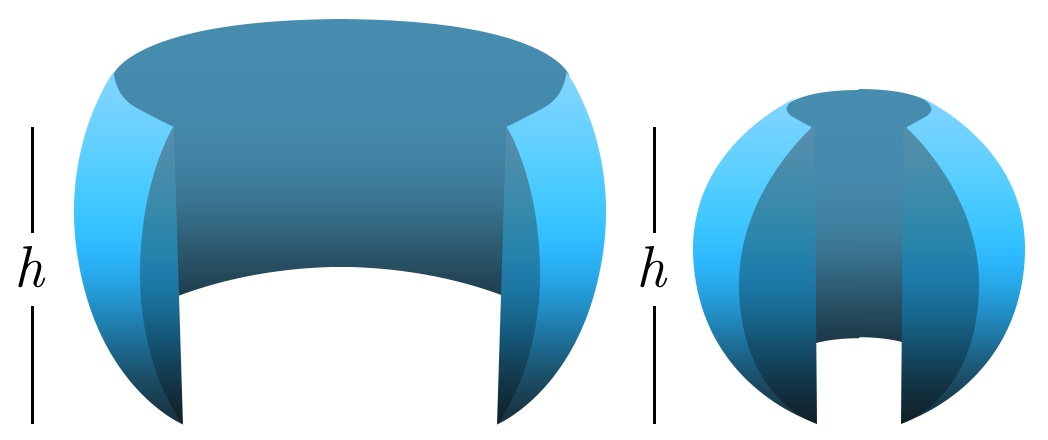
\includegraphics{napkin-ring.png}
  \end{center}
\end{probboxed}

We'll compare two different rings of the same height, and show that they have the same volume. This will mean that the original radius doesn't matter. To show this, we'll use \emph{Cavalieri's principle}. Imagine two identical stacks of coins, side-by-side:
\begin{center}
  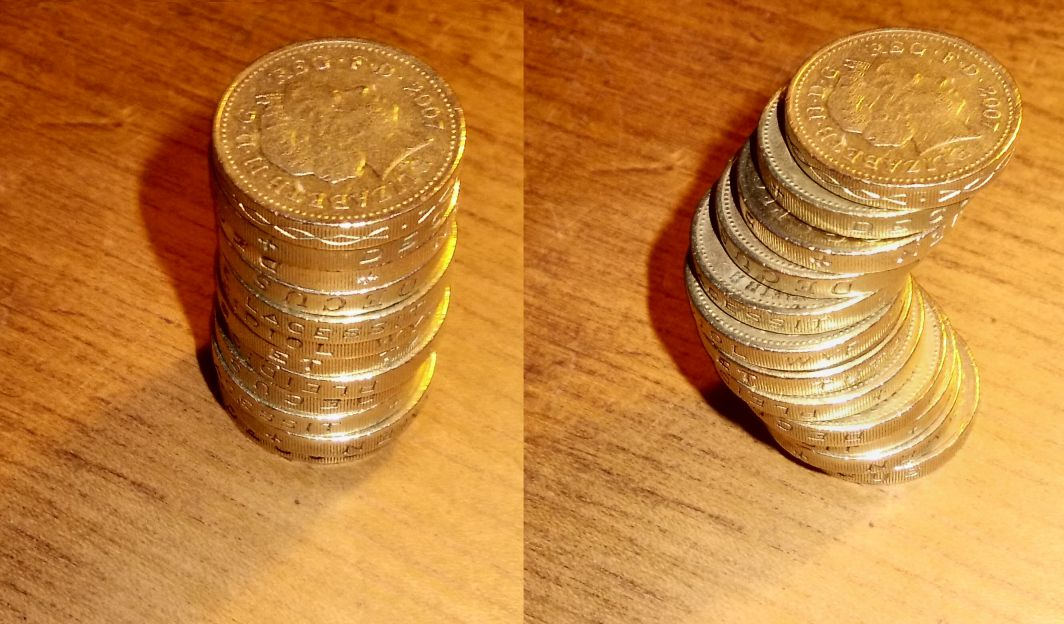
\includegraphics[width=8cm]{cavalieri-coins.JPG}

  {\sffamily \footnotesize Photo by \href{https://commons.wikimedia.org/wiki/File:Cavalieri\%27s_Principle_in_Coins.JPG}{Chiswick Chap}, CC BY-SA 3.0.}
\end{center}

Consider a plane parallel to the floor that intersects both stacks. The cross-section for both stacks is a circle. The two circles have the same area, the area of a single coin. Even if you move the plane higher or lower, the two cross-sections will always have the same area. Because of this, we know that both stacks have the same volume.

This is essentially Cavalieri's principle. Suppose you have two solids, and a plane intersecting both. \bluebf{If the area of the two cross-sections is the same, for any parallel plane, then the solids have the same volume.}

Cavalieri's principle looks like a good approach for this problem, as both solids have the same height. We need to show that the cross-sections have the same area.

\begin{exboxed}
  Suppose you have two rings of heights $h$, with radii $R$ and $r$, side-by-side on the ground. Consider a plane parallel to the ground intersecting both rings.
    \begin{enumthin}
      \item[(a)] What are the shapes of the cross-sections?
      \item[(b)] Suppose that this plane is height $x + \frac h2$ above the ground. What are the areas of both cross-sections? \hints{\ref{h:np01} \ref{h:bf11}}
    \end{enumthin}
\end{exboxed}

\begin{center}
  
\includegraphics[width=12cm]{napkin-ring-2.png}
\end{center}

If we draw a plane parallel to the ground intersecting a ring, the region formed is an annulus. So to find its area, we need to find its larger and smaller radii.

How will we find the length of its larger radius? We somehow need to use the radius of the original sphere. If we draw a larger radius, and connect both endpoints to the center of the sphere, we notice that it forms a right triangle!

\begin{minipage}{.5\textwidth}
  \begin{center}
    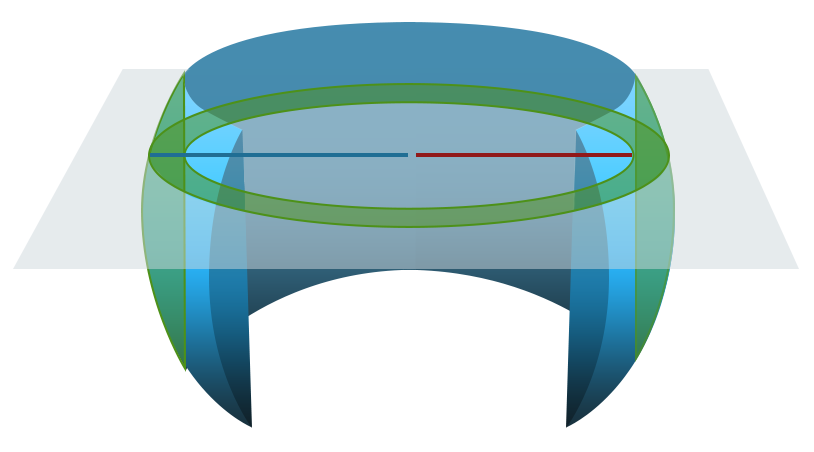
\includegraphics[width=8cm]{napkin-ring-3.png}
  \end{center}
\end{minipage}
\begin{minipage}{.5\textwidth}
  \begin{center}
    \begin{asy}
      size(5cm);
      real x = 10;
      real y = sqrt(13*13 - x*x);
      real x2 = 12;
      real y2 = sqrt(13*13 - x2*x2);
      draw(circle((0,0), 13));
      unfill((x, 15)--(x, -15)--(-x, -15)--(-x, 15)--cycle);
      fill(ellipse((0, y2), x2, 3), opacity(0.2)+greeny);
      unfill(ellipse((0, y2), x, 2));
      //draw(ellipse((0, y2), x, 2), greeny);
      //draw(ellipse((0, y2), x2, 3), greeny);
      draw((x, y)--(x, -y));
      draw((-x, y)--(-x, -y));
      draw((-x2, y2)--(0, y2)--(0, 0)--cycle, bluey);
      draw((0, 0)--(0, -y)--(x, -y)--cycle, ruddy);
      draw((0, y2)--(x, y2), ruddy);
      label("$R$", (-x2, y2)--(0, 0), S);
      label("$x$", (0, y2)--(0,0), E);
      label("$\frac12h$", (0,0)--(0, -y), W);
      label("$R$", (0, 0)--(x, -y), N+(0,0.5));
      //unfill(circle((0.3, y2), 0.3));
    \end{asy}
  \end{center}
\end{minipage}

In the figure, this right triangle is drawn as blue. By the Pythagorean theorem, we get the length of the larger radius as $\sqrt{R^2 - x^2}$. However, we can't do the same thing for the smaller radius, because we don't know the hypotenuse.

But notice that the smaller radius is also the radius of the cylinder drilled through the sphere! So drawing the radius at the bottom gives us a right triangle we can work with. The shorter radius is $\sqrt{R^2 - \del{\frac12h}^2}$, so the area of the annulus is $$\pi\del{\sqrt{R^2 - \del{\frac12 h}^2}}^2 - \pi\del{\sqrt{R^2 - x^2}}^2 = \pi\del{\del{\frac12 h}^2 - x^2}.$$

We can repeat the calculation for the second ring, but we can do something clever. Note that this area doesn't depend on $R$ at all! So if we repeat the computation for the second ring, we would get the same thing.

By Cavalieri's principle, we can conclude that the volume of a napkin ring depends only on its height. Try to finish the proof by finding its actual volume:

\begin{exboxed}
  Compare the ring to a sphere of height $h$.
  \begin{enumthin}
    \item[(a)] Show that the volumes of the ring and the sphere the same. \hint{\ref{h:np03}}
    \item[(b)] Conclude that the volume of the ring is $\frac16\pi h^3$.
  \end{enumthin}
\end{exboxed}

\vspace{-10pt}

\begin{mdframed}[style=exmdbox]
  \begin{problem}[\faBolt]
  \label{pr:spherecone}
  Without using the formula for the volume of a sphere, show that the volumes of the first two solids add up to the volume of the third:
    \begin{enumthin}
      \item[(a)] half of a sphere with radius $r$,
      \item[(b)] a cone of height $r$, whose base has radius $r$, and
      \item[(c)] a cylinder of radius $r$ and height $r$. \hints{\ref{h:np11} \ref{h:np12} \ref{h:np13}}
    \end{enumthin}
  \end{problem}
  \begin{problem}[\faBolt\,\faBolt \! \cite{reedcavalieri}]
    A \emph{cycloid} is the curve traced by a point on the circumference of a circle as it rolls along a straight line without slipping. Find the area underneath a cycloid. The following diagram might help. \hints{\ref{h:np21} \ref{h:np22} \ref{h:np23}}
    \begin{center}
      \begin{asy}
        import graph;
        size(4cm);
        pair F(real t) {
        return (t - sin(t), 1 - cos(t));
        }
        path g = graph(F, 0, pi);
        path h = rotate(180,(pi/2, 1))*g;
        pair O = (1, 1);
        path c = circle(O, 1);
        pair A = intersectionpoints(g, c)[0];
        pair B = intersectionpoints(h, c)[0];
        fill(g--(pi,0)--cycle, opacity(0.2)+bluey);
        draw(g^^h^^c);
        draw((0, 0)--(pi, 0));
        draw((0, 2)--(pi, 2));
        draw(A--B);
        dot(A^^B);
      \end{asy}
    \end{center}
  \end{problem}
\end{mdframed}

% \begin{problem}
  % Cavalieri's principle also has a two-dimensional 
  %  n reed's area of a cycloid
% \end{problem}

\subsection{Pappus's centroid theorem}

To talk about the next theorem, we need to define what a \emph{centroid} is.

\begin{exboxed}
  A plate of uniform thickness is in the shape of a triangle. Its vertices have coordinates $(1, 0)$, $(5, 3)$, and $(6, 0)$. The plate is on top of a thin pole. At which point on the plate should the pole be under so the plate stays balanced?
  \begin{center}
    \begin{asy}
      size(12cm);
      transform t = yscale(0.7)*shift(-5, 0);
      pair A = t*(1, 0);
      pair B = t*(5, 3);
      pair C = t*(6, 0);
      pair G = (A+B+C)/3;
      draw(G--(G-(0,3)));
      filldraw(A--B--C--cycle, opacity(0.2)+bluey, bluey);
      label("$(1, 0)$", A, 2N);
      label("$(5, 3)$", B, N);
      label("$(6, 0)$", C, 2N+E);

      filldraw(t*(8, 0)--t*(8, 3)--t*(12, 3)--t*(12, 0)--cycle, opacity(0.2)+bluey, bluey);
      draw(t*(10, 1.5)--(t*(10, 1.5) - (0, 3)));

      filldraw(t*circle((15, 1.5), 1.5), opacity(0.2)+bluey, bluey);
      draw(t*(15, 1.5)--(t*(15, 1.5) - (0, 3)));

      filldraw(t*(17, 0)--t*(20, 3)--t*(23, 0)--cycle, opacity(0.2)+bluey, bluey);
      draw(t*(20, 1)--(t*(20, 1) - (0, 3)));
    \end{asy}
  \end{center}
\end{exboxed}

Let's think about where this point would be for different shapes of plates. The point should have some kind of symmetry around it. For example, for a rectangle or circle, the point would lie on its center. For an isosceles triangle, it should lie on its axis of symmetry. It's some kind of center.

This point is called the \bluebf{centroid} of the region. For triangles, it lies on the centroid of the triangle, which we can find just by averaging its coordinates. In this case, we get the centroid's coordinates as $\del{\frac13\del{1+5+6}, \frac13\del{0+3+0}}$, or $\del{4, 1}$:

\begin{center}
  \begin{asy}
    size(3.5cm);
    transform t = yscale(0.7)*shift(-5, 0);
    pair A = t*(1, 0);
    pair B = t*(5, 3);
    pair C = t*(6, 0);
    pair G = (A+B+C)/3;
    draw(G--(G-(0,3)));
    filldraw(A--B--C--cycle, opacity(0.2)+bluey, bluey);
    label("$(4, 1)$", G, N);
  \end{asy}
\end{center}

One use of centroids is Pappus's centroid theorem, which we will not prove:

\begin{thmboxed}[Pappus's centroid theorem]
  Consider the solid of revolution formed by rotating a figure about an axis. Its volume is the product of the area of the figure and the distance traveled by its centroid.
\end{thmboxed}

\begin{center}
  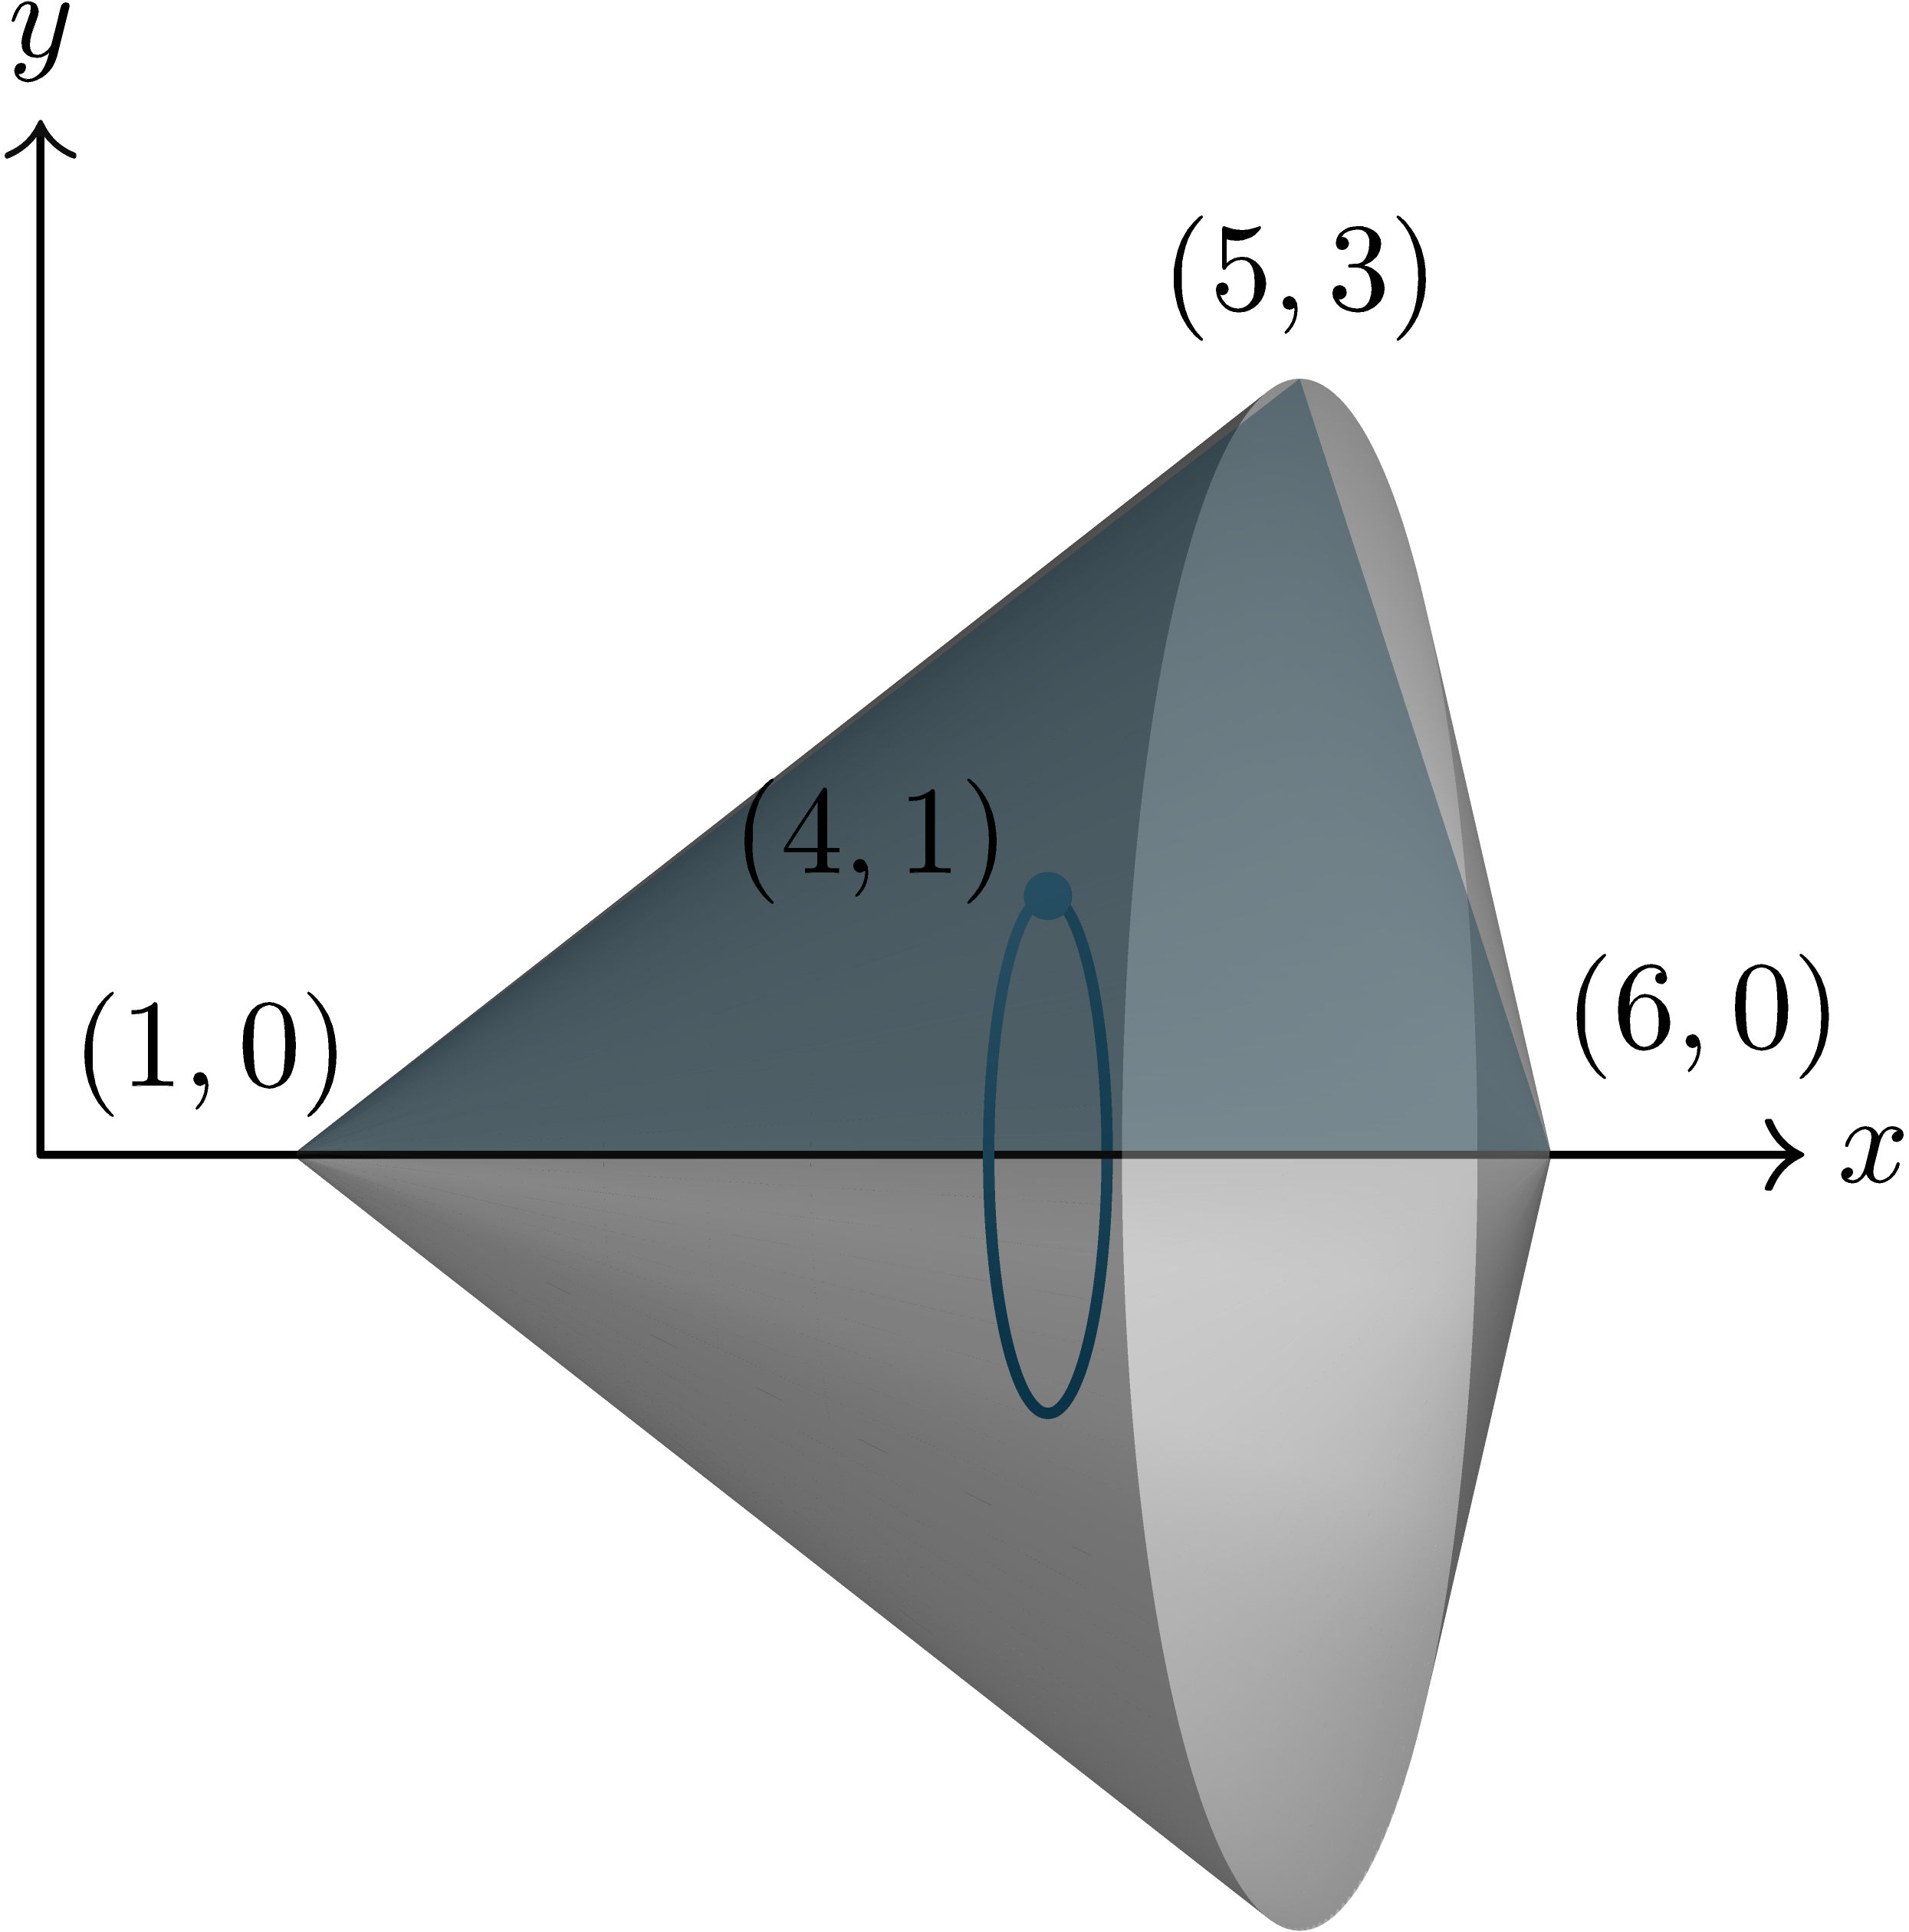
\includegraphics{3d1.png}
\end{center}

A \bluebf{solid of revolution} is the solid traced out by rotating the figure around an axis. The above shows the solid formed by rotating the triangular plate about the $x$-axis. The centroid is distance $1$ from the $x$-axis, so it travels a distance of $2\pi$. The triangle has area $7.5$, so the solid's volume is $15\pi$.

\begin{exboxed}
  Check that its volume is $15\pi$ by dividing the solid into two cones.
\end{exboxed}

To find the volumes of other solids of revolution, we need to be able to find the centroid of other shapes. We'll focus on polygons in this handout. Our strategy is to \bluebf{divide a polygon into triangles and rectangles}. For example:

\begin{exboxed}
  Consider the trapezoid with coordinates $(0, 0)$, $(9, 0)$, $(6, 4)$, and $(0, 4)$.
  \begin{center}
    \begin{asy}
      size(4cm);
      draw((0, 0)--(6, 0)--(6, 4)--(0, 4)--cycle);
      draw((6, 0)--(9, 0)--(6, 4));
      label("$(0,0)$", (0,0), S);
      label("$(9,0)$", (9,0), S);
      label("$(6,4)$", (6,4), N);
      label("$(0,4)$", (0,4), N);
      dot((19/5, 28/15));
    \end{asy}
  \end{center}
  \begin{enumthin}
    \item[(a)] Divided as above, find the centroids and areas of the rectangle and triangle.
    \item[(b)] Find the centroid of the trapezoid.
  \end{enumthin}
\end{exboxed}

The rectangle has centroid $(3, 2)$ and area $24$, while the triangle has centroid $\del{7, \frac43}$ and area $6$. To find the centroid, \bluebf{take the average of the centroids of each part, weighted by that part's area}. This means multiplying the coordinates by their areas, taking their sum, then dividing by the total area, for each coordinate:
$$\del{\frac{3 \cdot 24 + 7 \cdot 6}{24 + 6}, \frac{2 \cdot 24 + \frac43 \cdot 6}{24 + 6}} = \del{\frac{19}5, \frac{28}{15}}.$$ 
\vspace{-12pt}
\begin{exboxed}
  Some questions about the above trapezoid:
  \begin{enumthin}
    \item[(a)] Divide it into two triangles by joining $(0, 0)$ and $(6, 4)$. Repeat the process for finding the centroid. Do you get the same point?
    \item[(b)] What is the volume of the solid formed by rotating it about the $x$-axis? Check the result by dividing the solid into a cylinder and a cone.
    \item[(c)] What is the volume of the solid formed by rotating it about the $y$-axis?
  \end{enumthin}
\end{exboxed}

Finally, a few notes on computing centroids:
\begin{enumerate}
  \item \bluebf{The centroid isn't always at the average of the coordinates!} Example: the above trapezoid. This is why we need to divide polygons.
  \item \bluebf{The centroid always lies on an axis of symmetry}. Example: If you have a shape that's symmetric about $x=0$, the $x$-coordinate of the centroid is $0$. The $y$-coordinate of the centroid stays the same even if you ignore the left half.
  \item You can find centroids of shapes with holes by considering the holes as having negative area. Check this with the above trapezoid: it's a rectangle with corners $(0, 0)$ and $(9, 4)$, with triangle $(6, 4)$, $(9, 4)$, $(9, 0)$ having negative area.
\end{enumerate}

\begin{mdframed}[style=exmdbox]
  \begin{exercise}
    If you don't know the formulas for the volumes of a cone or cylinder, derive them. If you do know them, check that they agree with Pappus's centroid theorem.
  \end{exercise}

  \begin{exercise}
    Two people, of weights $40 \text{ kg}$ and $50 \text{ kg}$, sit on either end of a seesaw with length $10\text{ m}$. Where should the center of the seesaw be placed to balance it? \hint{\ref{h:pc21}}
  \end{exercise}

  \begin{problem}
    The formula for the volume of a sphere is $\frac43\pi r^3$, where $r$ is the radius. Where is the centroid located on a semicircle of radius $r$? \hint{\ref{h:pc31}}
  \end{problem}

  \begin{problem}[\faBolt]
    The solid formed when the previous trapezoid is rotated about the $y$-axis is called a \emph{frustrum}. It is what you get when you take a cone, and cut it with a plane parallel to its base. The formula for the volume of a frustrum is $\frac13\pi h\del{R^2 + Rr + r^2}$, where the height of the frustrum is $h$ and the radii of the bases are $r$ and $R$. 
    \begin{enumthin}
      \item Check that this formula gives the same volume you computed for the previous trapezoid.
      \item Prove that the formula is true using Pappus's centroid theorem. \hint{\ref{h:pc41}}
      \item Prove that the formula is true in a different way, by considering a frustrum as the difference between two cones. \hints{\ref{h:pc42} \ref{h:pc43} \ref{h:pc44}}
    \end{enumthin}
  \end{problem}

  \begin{problem}[\faBolt\,\faBolt \! \href{http://cjquines.com/files/sipnayan2017shs.pdf}{Sipnayan 2017}]
    A credit card has the shape of a $3 \times 4$ rectangle. If you rotate the card about one of its diagonals, what is the volume of the resulting solid of revolution? \hints{\ref{h:pc50} \ref{h:pc51} \ref{h:pc52} \ref{h:pc53}}
  \end{problem}
\end{mdframed}

% defer formal proof to appendix

\section{Metric relationships}

This final section is about metric relationships. In geometry, we use the word ``metric'' to describe anything involving length. Here, we talk about two very different theorems: one of them involves four circles, and the other involves quadrilaterals and their diagonals.

\subsection{Descartes' theorem}

Try solving the following problem using the Pythagorean theorem:

\begin{probboxed}
  Two unit circles are externally tangent to each other and internally tangent to a larger circle of radius $2$. A fourth circle is externally tangent to both smaller circles and internally tangent to the larger circle. What is its radius?

  \begin{center}
    \begin{asy}
      size(4cm);
      pair A = (1, 0);
      pair B = (0, 0);
      pair C = (0, 4/3);
      draw(circle(B, 2));
      draw(circle(A, 1));
      draw(circle(B-A, 1));
      draw(circle(C, 2/3));
    \end{asy}
  \end{center}
\end{probboxed}

Label the points as in the figure below, noting that $\angle ABC$ is a right angle. Let the radius of the fourth circle be $r$. Then $AB$ is $1$, $AC$ is $1 + r$ because it the sum of the radii of circle $A$ and circle $C$, and $BC$ is $2 - r$ because it is the difference of the radii of the circle $B$ and circle $C$.

\begin{center}
  \begin{asy}
    size(4cm);
    pair A = (1, 0);
    pair B = (0, 0);
    pair C = (0, 4/3);
    draw(circle(B, 2));
    draw(circle(A, 1));
    draw(circle(B-A, 1));
    draw(circle(C, 2/3));
    draw(A--B--C--cycle);
    draw(C--(0, 2));
    label("$A$", A, E);
    label("$B$", B, W);
    label("$C$", C, W);
  \end{asy}
\end{center}

By the Pythagorean theorem, we get $r^2 + (2 - r)^2 = (1 + r)^2$. We find that $r = \frac23$. Descartes' theorem directly solves problems like these, without setting up anything:

\begin{thmboxed}[Descartes' theorem]
  Let $k_1$, $k_2$, $k_3$, and $k_4$ be the curvatures of four circles, each tangent to the other three. Then $\del{k_1 + k_2 + k_3 + k_4}^2 = 2(k_1^2 + k_2^2 + k_3^2 + k_4^2)$.
\end{thmboxed}

To use it, we need to define \bluebf{curvature}. If two externally tangent circles have radii $r_1$ and $r_2$, their curvatures are $\frac1{r_1}$ and $\frac1{r_2}$. If one circle is internally tangent, the inner circle's curvature is still $\frac1{r_1}$, while the outer circle has curvature $-\frac1{r_2}$.

\begin{center}
  \begin{asy}
    size(6cm);
    draw(circle((0, 0), 3));
    draw(circle((5, 0), 2));
    draw(circle((11, 0), 3));
    draw(circle((12, 0), 2));
    label("$\frac13$", (0, 0));
    label("$\frac12$", (5, 0));
    label("$-\frac13$", (9, 0));
    label("$\frac12$", (12, 0));
  \end{asy}
\end{center}

In the figure, the circles are labeled with their curvature. Think of it this way: smaller circles bend more sharply, so they have higher curvature.

\begin{exboxed}
  Try applying Descartes' theorem to the above problem. Note that the outer circle's curvature is negative!
\end{exboxed}

The curvature of the two inner circles are both $1$, while the curvature of the outer circle is $-\frac12$. Substituting and solving, we get
\begin{align*}
  \del{1 + 1 - \frac12 + k_4}^2 &= 2\del{1^2 + 1^2 + \del{-\frac12}^2 + k_4^2} \\
  k_4^2 + 3k_4 + \frac94 &= \frac92 + 2k_4^2 \\
  4k_4^2 - 12k_4 + 9 &= 0.
\end{align*}
The last equation factors as $\del{2k_4 - 3}^2 = 0$, so we get $k_4 = \frac32$. Its radius must be its reciprocal, or $\frac23$. Remember to take the reciprocal to get the radius! One last thing:

\begin{exboxed}
  Note that curvatures $1$, $1$, $4$, and $0$ satisfy Descartes' theorem. What does this correspond to geometrically?
\end{exboxed}

A curvature of $0$ looks like it would belong to a circle of infinite radius, like a line. Which makes sense: a line doesn't curve, so it would have curvature $0$. Indeed, circles of radii $1$, $1$, and $\frac14$ are externally tangent to a line:

\begin{center}
  \begin{asy}
    size(4cm);
    draw(circle((0, 1), 1));
    draw(circle((2, 1), 1));
    draw(circle((1, 1/4), 1/4));
    draw((-1, 0)--(3, 0));
  \end{asy}
\end{center}

This gives us a useful special case for Descartes' theorem: \bluebf{one of the circles can be a line, which has zero curvature}. The equation still applies.

\begin{mdframed}[style=exmdbox]
  \begin{exercise}
    Three unit circles are externally tangent to each other and internally tangent to a circle of radius $R$. Find $R$.
  \end{exercise}

  \begin{exercise}
    \label{pr:descartesformula}
    Solve the equation in Descartes' theorem for $k_4$. What happens when $k_3 = 0$?
  \end{exercise}

  \begin{problem}[\faBolt \! \href{https://artofproblemsolving.com/wiki/index.php/2015_AMC_12A_Problems/Problem_25}{AMC 12A 2015}]
    A collection of circles in the upper half-plane, all tangent to the $x$-axis, is constructed in layers as follows. Layer $L_0$ consists of two circles of radii $70^2$ and $73^2$ that are externally tangent. For $k\geq 1$, the circles in $\textstyle\bigcup_{j=0}^{k-1} L_j$ are ordered according to their points of tangency with the $x$-axis. For every pair of consecutive circles in this order, a new circle is constructed externally tangent to each of the two circles in the pair. Layer $L_k$ consists of the $2^{k-1}$ circles constructed in this way. Let $S=\textstyle\bigcup_{j=0}^6 L_j$, and for every circle $C$ denote by $r(C)$ its radius. What is \[\sum_{C\in S}\dfrac1{\sqrt{r(C)}}?\]
    \begin{center}
      \begin{asy}
      size(8cm);
      // define a bunch of arrays and starting points
      pair[] coord = new pair[65];
      int[] trav = {32,16,8,4,2,1};
      coord[0] = (0,73^2); coord[64] = (2*73*70,70^2);
      // draw the big circles and the bottom line
      path arc1 = arc(coord[0],coord[0].y,260,360);
      path arc2 = arc(coord[64],coord[64].y,175,280);
      fill((coord[0].x-910,coord[0].y)--arc1--cycle,bluey+opacity(0.2));
      fill((coord[64].x+870,coord[64].y+425)--arc2--cycle,bluey+opacity(0.2));
      draw(arc1^^arc2);
      draw((-930,0)--(70^2+73^2+850,0));
      // We now apply the findCenter function 63 times to get
      // the location of the centers of all 63 constructed circles.
      // The complicated array setup ensures that all the circles
      // will be taken in the right order
      for(int i = 0;i<=5;i=i+1)
      {
      int skip = trav[i];
      for(int k=skip;k<=64 - skip; k = k + 2*skip)
      {
      pair cent1 = coord[k-skip], cent2 = coord[k+skip];
      real r1 = cent1.y, r2 = cent2.y, rn=r1*r2/((sqrt(r1)+sqrt(r2))^2);
      real shiftx = cent1.x + sqrt(4*r1*rn);
      coord[k] = (shiftx,rn);
      }
      // Draw the remaining 63 circles
      }
      for(int i=1;i<=63;i=i+1)
      {
      filldraw(circle(coord[i],coord[i].y),bluey+opacity(0.2));
      }
      \end{asy}
    \end{center}
    \hints{\ref{h:dt31} \ref{h:dt32}}
  \end{problem}

  \begin{problem}[\faBolt\,\faBolt \! \href{https://services.artofproblemsolving.com/download.php?id=YXR0YWNobWVudHMvYi84LzAwNWQ1ZDMzMmNlZmNhMmRiM2Q3YTg2YmVhZDE5NjFmYmIwYjUz\&rn=MjAxMGNvbnRlc3RlbnRpcmVkcmFmdHYxLjQucGRm}{ARML 2010}]
    Let $\varphi = \frac{1 + \sqrt5}2$ and let $\rho = \varphi + \sqrt{\varphi}$.
    \begin{enumthin}
      \item[(a)] Prove that $\rho^4 = 2\rho^3 + 2\rho^2 + 2\rho - 1$. \hints{\ref{h:dt21} \ref{h:dt22}}
      \item[(b)] Show that four pairwise externally tangent circles with distinct radii in geometric progression must have common ratio $\rho$. \hints{\ref{h:dt23} \ref{h:dt24}}
    \end{enumthin}
  \end{problem}

  \begin{problem}[\faBolt\,\faBolt \! \href{https://en.wikipedia.org/wiki/Ford_circle}{Ford circles}]
    Let $C_1$ and $C_2$ be circles with centers $\del{\frac01, \frac12}$ and $\del{\frac11, \frac12}$, both tangent to the $x$-axis.
    \begin{enumthin}
      \item[(a)] Let $C_3$ be the circle tangent to $C_1$, $C_2$, and the $x$-axis. What is its radius? Its center?
      \item[(b)] Let $C_4$ be the circle tangent to $C_1$, $C_3$, and the $x$-axis. What is its radius? Its center?
      \item[(c)] Circles $C_1$, $C_2$, $C_3$, and $C_4$ are called \emph{Ford circles}. Show that there is a Ford circle with $x$-coordinate $q$, for every rational number $r$ between $0$ and $1$. \hints{\ref{h:dt41} \ref{h:bf11} \ref{h:dt42}}
      \item[(d)] If $r = \frac pq$, where the GCD of $p$ and $q$ is $1$, show that this circle has radius $\frac1{2q^2}$. \hint{\ref{h:dt43}}
    \end{enumthin}
  \end{problem}
\end{mdframed}

% defer formal proof to appendix

\subsection{Parallelogram law}

To prove our next theorem, we first need to show its special case for parallelograms:

\begin{probboxed}[Parallelogram law]
  In a parallelogram, the sum of the squares of the sides is the sum of the squares of the diagonals.
\end{probboxed}

There's a short proof of this using vectors. The theorem is equivalent to proving $2\norm{\mathbf x}^2 + 2\norm{\mathbf y}^2 = \norm{\mathbf x + \mathbf y}^2 + \norm{\mathbf x - \mathbf y}^2$. (Why?) Then a short proof follows by expanding the right-hand side using the dot product.

We will try proving the problem without using vectors. Since we have the squares of side lengths and their sums, we're encouraged to use the law of cosines. 

\begin{center}
  \begin{asy}
    size(4cm);
    pair A = (0, 0);
    pair B = (5, 0);
    pair D = (3, 4);
    pair C = B+D-A;
    draw(A--B--C--D--cycle^^A--C^^B--D);
    label("$A$", A, SW);
    label("$B$", B, SE);
    label("$C$", C, NE);
    label("$D$", D, NW);
  \end{asy}
\end{center}

Label the parallelogram $ABCD$. By the law of cosines on triangle $BAD$, we get $BD^2 = AB^2 + AD^2 - 2 \cdot AB \cdot AD \cdot \cos \angle BAD$. Again by the law of cosines on triangle $ADC$, we get $AC^2 = AD^2 + CD^2 - 2\cdot AD \cdot CD \cdot \cos \angle ADC$. But $\angle BAD$ and $\angle ADC$ are supplementary, meaning their cosines are negatives of each other. Add them to get
\begin{align*}
  BD^2 &= AB^2 + AD^2 - 2 \cdot AB \cdot AD \cdot \cos \angle BAD \\
  AC^2 &= BC^2 + CD^2 + 2\cdot AB \cdot AD \cdot \cos \angle BAD \\
  BD^2 + AC^2 &= AB^2 + BC^2 + CD^2  + AD^2,
\end{align*}
where we also used $AB = CD$ and $BC = AD$.

\begin{mdframed}[style=exmdbox]
  \begin{exercise}
    What happens when we apply the parallelogram law to a rectangle?
  \end{exercise}

  \begin{exercise}
    Try proving the parallelogram law using coordinates. Let the vertices be $(0, 0)$, $(a, 0)$, $(a + b, c)$, and $(b, c)$. Solve for the diagonals and sides using the distance formula.
  \end{exercise}

  \begin{problem}[\href{https://en.wikipedia.org/wiki/Apollonius\%27s_theorem}{Apollonius's theorem}]
    Let $D$ be the midpoint of side $BC$ in triangle $ABC$. Prove that $AB^2 + AC^2 = 2\del{AD^2 + BD^2}$. \hint{\ref{h:pl31}}
  \end{problem}

  \begin{problem}[\href{https://en.wikipedia.org/wiki/Stewart\%27s_theorem}{Stewart's theorem}]
    Let $D$ be a point on side $BC$ of triangle $ABC$. Prove that $AB^2 \cdot DC + AC^2 \cdot BD = BD \cdot DC \cdot BC + AD^2 \cdot BC.$ \hint{\ref{h:pl41}}
  \end{problem}
\end{mdframed}

\subsection{Euler's quadrilateral theorem}

We end with Euler's quadrilateral theorem, a generalization of the parallelogram law:

\begin{thmboxed}[Euler's quadrilateral theorem]
  In a quadrilateral with sides $a$, $b$, $c$, and $d$, diagonals $e$ and $f$, and $g$ the length of the segment joining the midpoints of the two diagonals, $a^2 + b^2 + c^2 + d^2 = e^2 + f^2 + 4g^2$.
\end{thmboxed}

\newpage

Before we begin proving it, let's first check if it makes sense:

\begin{exboxed}
  Check that Euler's quadrilateral theorem makes sense when applied to a parallelogram.
\end{exboxed}

We will present Euler's original proof of this fact. It is a delightful proof in the spirit of the handout \href{http://cjquines.com/files/constructions.pdf}{Constructions}, involving, of course, constructing a parallelogram!

\begin{exboxed}
  In quadrilateral $ABCD$, let $P$ and $Q$ be the midpoints of $AC$ and $BD$, respectively. Let $E$ be the point such that the midpoint of $BE$ is $P$. \begin{enumthin}
    \item[(a)] Show that proving $AB^2 + BC^2 + CD^2 + DA^2 = AC^2 + BD^2 + DE^2$ is equivalent to proving the theorem. \hint{\ref{h:eq01}}
    \item[(b)] Let $F$ be the point such that the midpoint of $DF$ is $P$. Identify three parallelograms, whose diagonals all pass through $P$.
    \item[(c)] Conclude by using the parallelogram law on these three parallelograms! \hint{\ref{h:eq02}}
  \end{enumthin}
\end{exboxed}

\begin{center}
  \begin{asy}
    size(7cm);
    pair A = (0, 0);
    pair B = (0.3, -1);
    pair C = (2.4, -1);
    pair D = (1, 0.7);
    pair P = (A+C)/2;
    pair Q = (B+D)/2;
    pair Ep = 2*P-B;
    pair F = 2*P-D;
    draw(A--B--C--D--cycle);
    draw(A--C^^B--D);
    draw(P--Q^^D--Ep);
    draw(A--Ep--F--A^^B--Ep--C--F--B^^D--F, linetype(new real[] {1,5}));
    label("$A$", A, NW);
    label("$B$", B, SW);
    label("$C$", C, SE);
    label("$D$", D, NW);
    label("$P$", P, NE);
    label("$Q$", Q, W+(0, 0.5));
    label("$E$", Ep, NE);
    label("$F$", F, S);
  \end{asy}
\end{center}

The first equation has $DE^2$ instead of $4PQ^2$. So we need to show that $DE^2 = 4PQ^2$, or $DE = 2PQ$. But this $P$ is the midpoint of $BE$ and $Q$ is the midpoint of $BD$, making $DE$ a midline of $\triangle BDE$, so this is true.

The brilliant move in this proof is constructing $F$. This point completes \emph{three} different parallelograms: $ADCF$, $BDEF$, and $ABCE$. Now we apply the parallelogram law to each of them, in order:
\begin{align*}
  2DA^2 + 2CD^2 &= AC^2 + DF^2 \\
  BE^2 + DF^2 &= 2BD^2 + 2DE^2 \\
  2AB^2 + 2BC^2 &= AC^2 + BE^2.
\end{align*}
Adding the three equations, canceling the $BE^2 + DF^2$ on both sides, and then dividing by $2$ gives the first equation. So we are done!

\begin{mdframed}[style=exmdbox]
  \begin{problem}
    What happens when $C$ is the midpoint of $BD$? More generally, what happens when $C$ is any point on segment $BD$?
  \end{problem}

  \begin{problem}
    If you're familiar with vectors, there's a particularly short proof using them. Consider vectors $\mathbf a$, $\mathbf b$, $\mathbf c$, and $\mathbf d$. Let $\mathbf p = \frac12\del{\mathbf a + \mathbf c}$ and $\mathbf q = \frac12\del{\mathbf b + \mathbf d}$. Then show that $$\norm{\mathbf b - \mathbf a}^2 + \norm{\mathbf c - \mathbf b}^2 + \norm{\mathbf d - \mathbf c}^2 + \norm{\mathbf a - \mathbf d}^2 = \norm{\mathbf c - \mathbf a}^2 + \norm{\mathbf d - \mathbf b}^2 + 4\norm{\mathbf q - \mathbf p}^2.$$ Does your proof work even when the vectors aren't coplanar? \hint{\ref{h:eq21}}
  \end{problem}

  \begin{problem}[\faBolt]
    In fact, the theorem is true for \emph{any four points in space}. Check this makes sense with the following four points on a rectangular prism, by finding the length of $PQ^2$ using Euler's quadrilateral theorem, and through another method. \hints{\ref{h:bf11} \ref{h:eq31} \ref{h:eq32}} % Find the length of $PQ^2$ using the three-dimensional version of the Pythagorean theorem.
    \begin{center}
      \begin{asy}
        size(5cm);
        pair A = (0, 0);
        pair B = (5, 2);
        pair D = (8, -2);
        pair H = (0, 8);
        pair C = B+D-A;
        pair E = H+D-A;
        pair G = B+H-A;
        pair F = C+H-A;
        pair P = (A+C)/2;
        pair Q = (D+F)/2;
        draw(A--B--C^^B--G, dotted+1);
        draw(P--Q, linetype(new real[]{6, 4}));
        fill(A--D--C--F--cycle, opacity(0.2)+bluey);
        draw(A--D--C--F^^D--F, bluey);
        draw(A--F^^A--C, bluey);
        draw(D--E--F--G--H--E^^A--H);
        label("$P$", P, S);
        label("$Q$", Q, (1, 0));
        label("$6$", G--H, NW);
        label("$8$", A--H, W);
        label("$10$", G--F, N);
      \end{asy}
    \end{center}
  \end{problem}

  \begin{problem}[\faBolt\,\faBolt]
    A regular tetrahedron has side length $2$. What is the length of the segment joining the midpoints of two edges that do not share a vertex? Can you find its length without using Euler's quadrilateral theorem? \hints{\ref{h:eq41} \ref{h:eq42} \ref{h:eq43}} %incredibly nice solution: a regular tetrahedron is a set of four non-adjacent vertices of a cube.
  \end{problem}
\end{mdframed}

\section{Grab bag}

These problems combine techniques in the handout, and are roughly sorted by difficulty. Recognizing what you need to use is an important skill.

\begin{mdframed}[style=exmdbox,frametitle={Grab bag}]
  \begin{problem}
    A rhombus with side length $1$ has diagonal $1.5$. What is the length of its other diagonal? \hints{\ref{h:gb81}}
  \end{problem}

  \begin{problem}[\cite{posameiter}]
    Prove that the sum of the lengths of the perpendiculars from any point on a side of a rectangle to the diagonals is constant. \hints{\ref{h:an42} \ref{h:gb72}} %CPIG
  \end{problem}

  \begin{problem}[\cite{prasolov2}]
    In tetrahedron $ABCO$, $\angle AOB$, $\angle BOC$, and $\angle COA$ are right. Prove that the segments connecting the midpoints of opposite edges are the same length. \hints{\ref{h:gb81} \ref{h:bf11} \ref{h:gbe3}}
  \end{problem} %euler's quad theorem and pythagorean theorem, pras 6.19

  \begin{problem}[\cite{prasolov1}]
    Points $D$, $E$, and $F$ lie on sides $BC$, $CA$, and $AB$ of $\triangle AB$ such that $DE$ and $DF$ are parallel to $AB$ and $AC$. Prove that $[ADEF]^2 = 4[BDF][CDE]$. \hint{\ref{h:rd62} \ref{h:gbx1}} %PRASOLOV 1.33
  \end{problem}

  \begin{problem}
    Let $O$ be a point on $\triangle ABC$ of tetrahedron $ABCD$. The line parallel to $DA$ passing through $O$ intersects $\triangle DBC$ at point $A_1$. Define $B_1$ and $C_1$ similarly. Prove that $$\frac{OA_1}{DA} + \frac{OB_1}{DB} + \frac{OC_1}{DC} = 1.$$ \hints{\ref{h:dg41} \ref{h:gb62} \ref{h:gbd3}}
  \end{problem}%pras 3.35, volumes!
\end{mdframed}

\begin{mdframed}[style=exmdbox,frametitle={},  frametitlebelowskip = 0pt,splittopskip = 0pt,  innertopmargin = 5pt,]
  \begin{problem}
    A circle has diameter $AB$. Let $C$ be the midpoint of one of the arcs $AB$, and $P$ any point on the opposite arc $AB$. Let $X$ and $Y$ be the feet of the perpendiculars from $A$ and $B$ to $CP$. Prove that $AX + BY = CP$. \hints{\ref{h:vs41} \ref{h:pt41}}
  \end{problem}

  \begin{problem}
    Point $O$ is inside regular hexagon $ABCDEF$. Prove that $[AOB] + [COD] + [EOF] = [BOC] + [DOE] + [FOA]$. \hints{\ref{h:gb81} \ref{h:gb82}}
  \end{problem} %PRAS4.28

  \begin{problem}[\faBolt]
    Let $A$ and $B$ be opposite vertices of a cube. Consider the triangle formed by the three vertices adjacent to $A$. Suppose $AB$ intersects this triangle at point $M$. What is the ratio of $AM$ to $AB$? \hints{\ref{h:gbc1} \ref{h:gbc2} \ref{h:gbc3}}
  \end{problem}%turn to 2d, pras 2.1

  \begin{problem}[\faBolt \! \cite{prasolov1}]
    On sides $BC$ and $CD$ of square $ABCD$ points $P$ and $Q$, respectively, are taken so that $\angle BAP = \angle PAQ$. Prove that $BP + QD = AQ$. \hints{\ref{h:pt41} \ref{h:pt42}}
  \end{problem} % pras 18.1

  \begin{problem}[\faBolt \! \cite{posameiter}]
    In parallelogram $ABCD$, $F$ is the midpoint of $AB$, and $E$ is the intersection of lines $BD$ and $CF$. If $[BEC] = 100$, find $[AFED]$. \hints{\ref{h:cv01} \ref{h:rd42}} %CPIG
  \end{problem}

  \begin{problem}[\faBolt \! \href{https://artofproblemsolving.com/wiki/index.php/1981_AHSME_Problems/Problem_19}{AHSME 1981}]
    In $\triangle ABC$, $M$ is the midpoint of side $BC$, $AN$ bisects $\angle BAC$, and $BN \perp AN$. If sides $AB$ and $AC$ have lengths $14$ and $19$, respectively, then find $MN$. \hints{\ref{h:gb61} \ref{h:gb62}}
  \end{problem}

  \begin{problem}[\faBolt\,\faBolt \! \cite{prasolov2}]
    A point $A$ is chosen inside a sphere of radius $R$. Three chords are drawn through $A$, each two of them perpendicular. If the lengths of the chords are $a$, $b$, and $c$, show that $a^2 + b^2 + c^2 = 12R^2 - 8x^2$, where $x$ is the distance from $A$ to the center of the sphere. \hints{\ref{h:bf11} \ref{h:eq31} \ref{h:gbb3} \ref{h:gbb4}}
  \end{problem}%pras 1.23

  \begin{problem}[\faBolt\,\faBolt]
    Prove that the area of a regular octagon is equal to the product of the lengths of its longest and shortest diagonals. \hints{\ref{h:os40} \ref{h:gb92}} %PRAS4.59
  \end{problem}

  \begin{problem}[\faBolt\,\faBolt \! \href{https://aops.com/community/c6h1525185}{JBMOSL 2014}]
    Let $ABC$ be a triangle with $\angle ABC = \angle BCA = 40^{\circ}$. The angle bisector of $\angle ABC$ meets side $AC$ at $D$. Prove that $BD + DA = BC$. \hints{\ref{h:gb31} \ref{h:gb32}}
  \end{problem}

  \begin{problem}[\faBolt\,\faBolt \! \cite{sayan}]
    Let $ABCDE$ be a convex pentagon with $AB = BC$ and $CD = DE$. If $\angle ABC = 2\angle CDE = 120\dg$ and $BD = 2$, find $[ABCDE]$. \hints{\ref{h:pl31} \ref{h:gba2} \ref{h:gba3} \ref{h:gba4}}
  \end{problem} % http://artofproblemsolving.com/community/c6h529620p3019876

  \begin{problem}[\faBolt\,\faBolt \! \cite{prasolov2}]
    In tetrahedron $ABCO$, $\angle AOB$, $\angle BOC$, and $\angle COA$ are right. Given that $OA = OB + OC$, prove that $\angle OAB + \angle BAC + \angle CAO = 90\dg$. \hints{\ref{h:gbc1} \ref{h:gbf2} \ref{h:gbf3} \ref{h:gbf4} \ref{h:gbf5}}
  \end{problem} %pras 6.21
\end{mdframed}

\section{Further reading}

On the sources of proofs: The proof of van Schooten's is original, as far as I know; the proof of Pompeiu's is on \cite{ctkvanschooten}; the proof of De Gua's is on \cite{bogomolnydegua}; the proof of Euler's is cited on \cite{sandifereuler}; the rest are well-known or on Wikipedia.

On the missing proofs: A good intuitive explanation of Pappus's centroid theorem is on \cite{brilliantpappus}. The Wikipedia page on \cite{wikipediapappus} has a rigorous proof. My favorite proof of Descartes's theorem is \cite{mutanguhadescartes}.

Viviani's theorem may seem simple on the surface, but \cite{abboudviviani} proves a lot of interesting extensions of it. The radiation symbol theorem's name is only used in \cite{weissteinradiation}; but \cite{gibertradiation} has some really interesting results about the configuration. 

There's this really cool animation of \autoref{pr:spherecone} on \cite{abelcavalieri}. Wikipedia has a short guide on computing centroids on \cite{wikipedialocating}, and a list of centroids of common shapes on \cite{wikipedialist}.

Using vectors in geometry is essentially like using complex numbers in geometry. My favorite introductory reference is \cite{egmo}; but \cite{chencomplex} is also great. The only reference I have specifically about vectors is \cite{livectors}.

If you liked the proofs of van Schooten's and Euler's quadrilateral, I will again link to my handout \href{http://cjquines.com/files/constructions.pdf}{Constructions}, which has more problems on the same themes.

\section{Hints}

Hints are in random order, so you don't accidentally glance at the next one.

\begin{enumthin}[leftmargin=0pt]
\item \label{h:gb92} Make a rectangle with side lengths the longest and shortest diagonals.
\item \label{h:os43} The rectangle is one-fourth of the area of the center region.
\item \label{h:vs01} Show that one of its angles is $60\dg$.
\item \label{h:pc44} Connect the tip of the cone to the centers of the bases, then draw parallel radii.
\item \label{h:dt43} It's equivalent to showing that $p$ doesn't matter when finding the radius.
\item \label{h:gbf5} $\triangle AOB \cong \triangle CRQ$, $\triangle AOC \cong \triangle BPQ$, hence $\triangle ABC \cong \triangle QCB$.
\item \label{h:pt54} Rotation carries $\triangle ABE$ to $\triangle BCD$; they have the same area. Use $\frac12 ab \sin C$.
\item \label{h:rt06} $x(xy+y+1)(yz+z+1) = x^2y^2z + x^2yz + x^2y + xy^2z + 2xyz + xy + xz + x$.
\item \label{h:vt41} One way to solve it: draw lines through $X$ parallel to the sides.
\item \label{h:rt41} Reduce computation by using symmetry.
\item \label{h:gbc1} Often, three-dimensional geometry problems can be turned to two-dimensional ones.
\item \label{h:pt32} Rotate $P$ $60\dg$ clockwise about each of $A$, $B$, and $C$. What's the area of the hexagon?
\item \label{h:np01} It remains to find the outer radius and the inner radius.
\item \label{h:pl41} The cosines of supplementary angles are negative. Find a way to eliminate them.
\item \label{h:os22} The shaded region is one-fourth of the area inside the grid but outside the circle.
\item \label{h:gba4} $\triangle FDE \cong \triangle BDC$. Arrange the remaining area to fit in $\triangle BDF$.
\item \label{h:vs03} Start by proving $B$, $D$, and $E_1$ are collinear, then prove $E_1$ lies on the circumcircle.
\item \label{h:dg42} Compute the volume with $\triangle AOB$ as a base, and with $\triangle ABC$ as a base. Equate.
\item \label{h:vt21} Choose $P$ strategically: it can be \emph{any} point.
\item \label{h:bf11} Use the Pythagorean theorem. 
\item \label{h:pc53} These coordinates work: $(-5/2, 0)$, $(5/2, 0)$, $(7/10, 12/5)$, $(0, 15/8)$, $(-7/10, 12/5)$.
\item \label{h:dt21} It might help to know $\varphi^2 = \varphi + 1$.
\item \label{h:rd43} Use coordinates.
\item \label{h:eq41} Applying the theorem isn't too bad: almost all the lengths are the same!
\item \label{h:gb31} Imitate our proof of van Schooten's theorem.
\item \label{h:pc42} Find the difference in the volumes of the cones. You need to find the height.
\item \label{h:np13} If it helps, remove an upside-down cone from the cylinder and use Cavalieri's.
\item \label{h:pt31} Do the same thing we did in the proof!
\item \label{h:gb81} This is nearly a direct application of one of the theorems discussed.
\item \label{h:dg31} The answer is not always. Try making $\triangle AOB$ equilateral and vary $OC$.
\item \label{h:vt42} If the sides of a triangle are doubled, its area must be quadrupled.
\item \label{h:vs04} Remember to make use of the fact that $BE$ and $PC$ are parallel!
\item \label{h:dt24} You have to show that the other roots of the polynomial aren't possible ratios.
\item \label{h:rd62} For similar triangles, the ratio of their areas is the square of the ratio of their lengths.
\item \label{h:gb61} Extend $BN$ to meet $AC$ at $Q$.
\item \label{h:pt01} Show that $\angle CBD = \angle ABP$.
\item \label{h:pc41} One way to set up coordinates is $(0, 0)$, $(0, R)$, $(r, h)$, $(0, h)$.
\item \label{h:dt32} If $S(n)$ is the sum in layer $n$, $S(n) = 2S(n-1) + 2S(n-2) + \cdots + S(0)$.
\item \label{h:vs41} Put the two segments together and hope it's congruent to the other segment.
\item \label{h:gb32} Choose a point $K$ on $BC$ such that $BD=BK$. $ADKB$ is cyclic.
\item \label{h:np12} If the sphere's base is flat on the floor, the cone's base should be pointing up.
\item \label{h:os42} The four corner regions are the same. The top and bottom regions are the same.
\item \label{h:pt51} Van Schooten's theorem looks like a good idea.
\item \label{h:gbb3} Look at the rectangular prism with opposite vertices at $A$ and the sphere's center.
\item \label{h:dt41} There's a nice formula for the $x$-coordinate of the between $a/b$ and $c/d$.
\item \label{h:gbf4} Construct point $Q$ such that $OPQR$ is a square.
\item \label{h:vt52} Place a regular polygon inside the equiangular one, such that the sides are parallel.
\item \label{h:eq01} You need to show $DE^2 = 4PQ^2$.
\item \label{h:rd42} One way to solve it: the centroid divides the triangle's median in the ratio $2 : 1$.
\item \label{h:dg52} Find $AB$, $BC$, $CA$ in terms of $AO$, $BO$, $CO$. Then find $[ABC]$ using Heron's.
\item \label{h:gbc3} View it from a perspective where $A$ and $B$ are opposite vertices of a rectangle.
\item \label{h:eq42} Consider a cube of side length $\sqrt2$.
\item \label{h:dt22} Find $\rho^2$, and use $\varphi^2 = \varphi + 1$. Find $\rho^3 = \rho^2 \cdot \rho$, and use $\varphi^2 = \varphi + 1$ again. Find $\rho^4$.
\item \label{h:pc31} Use Pappus's centroid theorem in reverse. And use symmetry.
\item \label{h:gb62} Similar triangles.
\item \label{h:vs42} Construct the point $P$ on ray $BT$ such that $TP = TC$. Then angle chase.
\item \label{h:gba3} $\triangle BDF$ is equilateral. Rearrange the area.
\item \label{h:rt52} Let's say $[BTD] = 1$. Find $[BTA]$ and $[ATE]$.
\item \label{h:an42} Look at the areas.
\item \label{h:eq02} You want to get rid of $BE^2$ and $DF^2$, so eliminate them. Like a system of equations.
\item \label{h:rd31} $\triangle APD \sim \triangle MPB$. In what ratio?
\item \label{h:np23} To explain why the segments are always equal, roll the two points along the curves.
\item \label{h:pc52} Set up coordinates so there's an axis of symmetry at $x = 0$. You only need to find $y$.
\item \label{h:np03} Nothing changes with our previous argument!
\item \label{h:an31} You're given the diameter, not the radius.
\item \label{h:gbe3} A nice solution: inscribe it in a rectangular prism. The length is half the longest diagonal.
\item \label{h:os41} Reflect the two perpendicular chords over the center of the circle. 
\item \label{h:vt51} Have you done \autoref{pr:vivianigeneralize}? Use it.
\item \label{h:pt53} Once you find $x$ and $y$, use the law of cosines on $\triangle ABD$.
\item \label{h:cv01} If two triangles have the same height, the ratio of their areas is the ratio of their bases.
\item \label{h:gbf3} Construct points $P$ and $R$ on rays $OB$ and $OC$ such that $OA = OP = OR$. 
\item \label{h:gb72} If the point is on side $AB$, and the diagonals meet at $E$, look at $[ABE]$.
\item \label{h:dt23} Let $r$ be the common ratio. Descartes' theorem gives a polynomial. $r^2 + 1$ is a factor.
\item \label{h:pc51} The shape you're rotating isn't a triangle, but like two mountain peaks.
\item \label{h:rt04} Use Menelaus's theorem. $AD$ is one of the triangle's sides.
\item \label{h:eq31} To find a certain length, use \autoref{pr:longestdiagonal}.
\item \label{h:gba2} Let $F$ be the point such that $ABEF$ is a paralellogram. Notice anything?
\item \label{h:pt42} Rotate $90\dg$ about $A$, then complete the triangle.
\item \label{h:pc43} Make similar right triangles to find the heights of the cones.
\item \label{h:rd52} This is similar to \autoref{pr:squarediagonal}.
\item \label{h:pc50} To get the shape you want, mirror the figure over the axis and ignore half of it.
\item \label{h:gbb4} If it has edges $d$ and $e$, then $(a/2)^2 = R^2 - (d^2 + e^2)$.
\item \label{h:vs32} Show that $\triangle CQA \sim \triangle PQB$, then use it.
\item \label{h:rt02} It's $[ARC]/[ADC]$ times $[ADC]/[ABC]$.
\item \label{h:cv02} What is $[ADB]/[CDA]$? What is $[PDB]/[CDP]$? Subtract.
\item \label{h:np22} You need to compare the lens-like shape and the circle.
\item \label{h:gbd3} If two pyramids have the same base, the ratio of their volumes is the ratio of their heights.
\item \label{h:eq32} Let $M$ be the midpoint of the common edge of the faces $P$ and $Q$. $\angle PMQ = 90\dg$.
\item \label{h:np11} Use Cavalieri's principle. Instead of the area of one cross-section, use the sum of two.
\item \label{h:rt05} Adding $1$ to $CD/BD$ gives $BC/BD$,
\item \label{h:pt52} Set $AD = x$, $BD = y$. Find the area of $ABE$ and $ACD$ in terms of $x$ and $y$.
\item \label{h:pc21} It's a one-dimensional centroid. You still take the weighted average.
\item \label{h:dt31} Did you solve \autoref{pr:descartesformula}? Rearrange the formula in terms of $1/\sqrt{r}$.
\item \label{h:rt03} You'll have to use another theorem. You have a lot of ratios here.
\item \label{h:vs31} Extend $PQ$ to meet the circumcircle again at $A$. What's special about $\triangle ABC$?
\item \label{h:gbc2} By viewing the cube at a certain angle, the triangle becomes a line.
\item \label{h:np21} Use Cavalieri's principle, but with two dimensions.
\item \label{h:os40} Draw some parallel lines to help rearrange the area.
\item \label{h:eq43} Four vertices of a cube, no two of them adjacent, form a regular tetrahedron.
\item \label{h:pt41} Rotate.
\item \label{h:gbf2} Rearrange the faces of the tetrahedron into a two-dimensional figure.
\item \label{h:pl31} All you have to do is construct a parallelogram.
\item \label{h:vs02} Show that both pairs of opposite sides are parallel.
\item \label{h:rd51} $\triangle ARQ \sim \triangle BSQ \sim \triangle DSC$. In what ratios?
\item \label{h:an41} No, they don't drain at the same rate.
\item \label{h:gb82} Extend $AB$, $CD$, $EF$ to make an equilateral triangle.
\item \label{h:dg41} Volume.
\item \label{h:dt42} The circle in between $x$-coordinates $a/b$ and $c/d$ has $x$-coordinate $(a+b)/(c+d)$.
\item \label{h:eq21} Use the fact that $\norm{\mathbf a}^2 = \mathbf a \bullet \mathbf a$.
\item \label{h:rt53} Draw $TC$. Let $[TDC] = x$, $[TEC] = y$. Use $AT/DT$, $BT/ET$ to find area ratios.
\item \label{h:gbx1} Find $[ADF]/[BDF]$. Use $AF = ED$.
\end{enumthin}

\begin{thebibliography}{99}
  \bibitem{abboudviviani} Abboud, E. On Viviani's Theorem and its Extensions. \url{https://arxiv.org/pdf/0903.0753.pdf}
  \bibitem{abelcavalieri} Abel, Z. Slicing Spheres. \url{http://blog.zacharyabel.com/2012/01/slicing-spheres/}
  \bibitem{bogomolnydegua} Bogomolny, A. Analogues and Generalizations of the Pythagorean Theorem. \url{https://www.cut-the-knot.org/Generalization/pythagoras.shtml}
  \bibitem{ctkvanschooten} Bogomolny, A. Van Schooten's and Pompeiu's Theorems. \url{http://www.cut-the-knot.org/Curriculum/Geometry/Pompeiu.shtml}
  \bibitem{brilliantpappus} Brilliant.org. Pappus's Centroid Theorems. \url{https://brilliant.org/wiki/pappus-centroid-theorems/}
  \bibitem{chencomplex} Chen, E. Bashing Geometry with Complex Numbers. \url{http://web.evanchen.cc/handouts/cmplx/en-cmplx.pdf}
  \bibitem{egmo} Chen, E. Euclidean Geometry in Mathematical Olympiads. \url{http://web.evanchen.cc/geombook.html}
  \bibitem{gibertradiation} Gibert, B. and van Lamoen, F. The Parasix Configuration and Orthocorrespondence. \url{http://forumgeom.fau.edu/FG2003volume3/FG200318.pdf}
  \bibitem{livectors} Li, K. Y. Vector Geometry. \url{http://www.math.ust.hk/excalibur/v6_n5.pdf}
  \bibitem{mutanguhadescartes} Mutanguha, J. P. From Heron's formula to Descartes' circle theorem. \url{http://eulerarchive.maa.org/hedi/HEDI-2005-01.pdf}
  \bibitem{posameiter} Posameiter, A. S. and Salkind, C. T. Challenging Problems in Geometry. \url{http://store.doverpublications.com/0486691543.html}
  \bibitem{prasolov1} Prasolov, V. Problems in Plane and Solid Geometry, Vol. 1, Plane Geometry. \url{http://e.math.hr/afine/planegeo.pdf}
  \bibitem{prasolov2} Prasolov, V. Problems in Plane and Solid Geometry, Vol. 2, Solid Geometry. \url{https://www.scribd.com/document/61948241/Viktor-v-Prasolov-Problems-in-Plane-and-Solid-Geometry-Vol-2-Solid-Geometry-239p}
  \bibitem{randiseventh} Randi, J. That Dratted Triangle. \url{https://web.archive.org/web/20060427055758/http://www.randi.org/jr/02-09-2001.html}
  \bibitem{reedcavalieri} Reed, N. Elementary proof of the area under a cycloid. Mathematical Gazette, volume 70, number 454, December, 1986, 290–291.
  \bibitem{sandifereuler} Sandifer, E. The Euler--Pythagoras theorem. \url{http://eulerarchive.maa.org/hedi/HEDI-2005-01.pdf}
  \bibitem{sayan} Sayan. Area of a convex pentagon. \url{http://artofproblemsolving.com/community/c6h529620p3019876}
  \bibitem{devilliersrouth} de Villiers, M. Feynman's Triangle: Some Feedback and More. \url{http://mysite.mweb.co.za/residents/profmd/feynman.pdf}
  \bibitem{weissteinradiation} Weisstein, E. W. Equal Parallelians Point. \url{http://mathworld.wolfram.com/EqualParalleliansPoint.html}
  \bibitem{weissteinrouth} Weisstein, E. W. Routh's Theorem. \url{http://mathworld.wolfram.com/RouthsTheorem.html}
  \bibitem{wikipediacavalieri} Wikipedia. Cavalieri's principle. \url{https://en.wikipedia.org/wiki/Cavalieri%27s_principle}
  \bibitem{wikipediaceva} Wikipedia. Ceva's theorem. \url{https://en.wikipedia.org/wiki/Ceva%27s_theorem}
  \bibitem{wikipediadescartes} Wikipedia. Descartes' theorem. \url{https://en.wikipedia.org/wiki/Descartes%27_theorem}
  \bibitem{wikipedialist} Wikipedia. List of centroids. \url{https://en.wikipedia.org/wiki/List_of_centroids}
  \bibitem{wikipedialocating} Wikipedia. Locating the center of mass. \url{https://en.wikipedia.org/wiki/Locating_the_center_of_mass}
  \bibitem{wikipediapappus} Wikipedia. Pappus's centroid theorem. \url{https://en.wikipedia.org/wiki/Pappus%27s_centroid_theorem}
  \bibitem{wikipediaparallelogram} Wikipedia. Parallelogram law. \url{https://en.wikipedia.org/wiki/Parallelogram_law}
  \bibitem{wikipediarouth} Wikipedia. Routh's theorem. \url{https://en.wikipedia.org/wiki/Routh%27s_theorem}
  \bibitem{wilsonviviani} Wilson, J. Equilateral Triangles and ``Viviani's Theorem''. \url{http://jwilson.coe.uga.edu/EMAT6680Su07/Gilbert/EMAT%206690/Viviani's%20Theorem/VivianiEssay.html}
\end{thebibliography}

If you spot a typo, see an error, have a suggestion, or want to ask a question, feel free to contact me at \mailto{cj@cjquines.com}.

\end{document}